\documentclass[11pt]{article}
\usepackage[margin=1in,top=0.85in,bottom=0.8in]{geometry}
\usepackage{fancyhdr}
\usepackage{booktabs}
\usepackage{amsmath,amssymb}
\usepackage{xcolor}
\usepackage{array}
\usepackage{multirow}
\usepackage{caption}
\usepackage{float}
\usepackage{graphicx}
\usepackage{longtable}
\usepackage{enumitem}
\usepackage{tabularx}
\usepackage{tikz}
\usetikzlibrary{arrows.meta, positioning, shapes.geometric, calc}

% ── Compact spacing ──
\setlength{\textfloatsep}{4pt plus 1pt minus 1pt}
\setlength{\floatsep}{4pt plus 1pt minus 1pt}
\setlength{\intextsep}{4pt plus 1pt minus 1pt}
\setlength{\abovecaptionskip}{3pt}
\setlength{\belowcaptionskip}{1pt}
\setlength{\parskip}{1.5pt plus 0.5pt}
\setlength{\parindent}{0pt}
\captionsetup{skip=2pt, font=small}

% ── Colors matching prior HW ──
\definecolor{secblue}{RGB}{0,90,170}

% ── Section formatting ──
\usepackage{titlesec}
\titleformat{\section}{\Large\bfseries\color{secblue}}{\thesection}{1em}{}
\titleformat{\subsection}{\large\bfseries}{\thesubsection}{1em}{}
\titleformat{\subsubsection}{\normalsize\bfseries}{\thesubsubsection}{1em}{}
\titlespacing*{\section}{0pt}{10pt}{3pt}
\titlespacing*{\subsection}{0pt}{6pt}{2pt}
\titlespacing*{\subsubsection}{0pt}{4pt}{1pt}

% ── Header/footer ──
\pagestyle{fancy}
\fancyhf{}
\fancyhead[L]{\small ISE 573 --- Assignment 10}
\fancyhead[R]{\small SodhiCable MES Design Prototype}
\fancyfoot[R]{\thepage}
\renewcommand{\headrulewidth}{0.4pt}
\renewcommand{\footrulewidth}{0pt}

% ── Overflow prevention ──
\emergencystretch=2em          % allow slightly looser lines rather than overflow
\tolerance=1200                   % tolerate wider word spacing before overflow

% ── Convenience ──
% \tfield allows line-breaks at underscores and dots in table.field names
\newcommand{\tfield}[1]{\texttt{\hyphenchar\font=`\-\relax #1}}
\newcolumntype{L}[1]{>{\raggedright\arraybackslash}p{#1}}

% ── Math formatting ──
\usepackage{tcolorbox}
\tcbuselibrary{skins,breakable}
\newtcolorbox{eqbox}[1][]{
  colback=secblue!3, colframe=secblue!40, boxrule=0.4pt,
  arc=2pt, left=6pt, right=6pt, top=4pt, bottom=4pt,
  fonttitle=\small\bfseries, title={#1},
  before upper={\parskip=2pt}
}

\begin{document}

% ── Title Block ──
\begin{center}
{\LARGE\bfseries SodhiCable MES Design Prototype\\[4pt]
Manufacturing Execution System for Wire \& Cable Production}\\[6pt]
{\large ISE 573 --- Manufacturing Execution Systems}\\[12pt]
\begin{tabular*}{\textwidth}{@{\extracolsep{\fill}}lcc r}
Stephen Eacuello & & ISE 573 --- Assignment 10 & April 2026
\end{tabular*}
\end{center}
\vspace{0.3em}
\hrule
\vspace{1.2em}

\begin{abstract}\noindent
This document presents the complete MES design prototype for SodhiCable, a multi-line wire and cable manufacturer operating 26 work centers across 15 equipment types, producing 33 products in 9 families for 20 customers spanning Defense, Infrastructure, Industrial, and Oil \& Gas segments.  The design implements all 11 MESA functions (F1--F11) in a 78-table SQLite schema with ${\sim}$25{,}000 lines of Python and a single dependency (Flask~3.0), exposing 244 REST API endpoints.  Each function is specified at the table-field level with full foreign-key annotations and accompanied by a mathematically formulated algorithm (LP, MILP, SPT/EDD, SPC $\bar{X}$-$R$/CUSUM/EWMA, PID, OEE, recursive CTE genealogy) traced to its ISE~573 course week and homework.  Beyond MESA-11, the prototype provides AI/ML integration via Claude API (natural-language-to-SQL queries, anomaly detection, predictive maintenance), pure-Python Isolation Forest and Gradient Boosted Stumps for anomaly detection and quality prediction, ISA-95 SCADA visualization with drill-down from Level~3 to Level~1, OPC-UA tag simulation, ERP Level 4 simulation with purchase orders, invoices, and ISA-95 B2MML messages, and 20 beyond-MESA functional modules including discrete event simulation, MRP with 7 lot-sizing methods, bottleneck analysis, and energy management.  A day-in-the-life integration timeline demonstrates cross-function event chains including quality alarms, maintenance events, and lot-level traceability.  Prototype validation against seeded production data confirms functional correctness (e.g., $C_{pk} = 0.87$ on DRAW-1 wire diameter, sub-10\,ms recall traces, downtime Pareto ranking).
\end{abstract}

%======================================================================
\section{System Overview}\label{sec:overview}
%======================================================================

\subsection{Business Context}

SodhiCable LLC is a mid-size specialty wire and cable manufacturer headquartered in Warwick, Rhode Island, founded circa 1988. With approximately 250 employees and \$80M in annual revenue, the company operates a single primary manufacturing facility (26 work centers, 69 equipment items, 150{,}000 sq.\ ft.) with one external processing partner (NJ-EXT for welded tube assemblies).

\textbf{Competitive Landscape:} Wire and cable manufacturing in North America is consolidating around tier-1 players: Prysmian/General Cable (\$16B global), Southwire (\$8B, largest US manufacturer), Encore Wire (\$2.5B, commodity building wire), and Belden (\$2.5B, specialty/industrial). Between 2015--2025, the top five manufacturers increased combined market share from 45\% to 62\%. Mid-size independents like SodhiCable compete on small-lot MTO agility, military certifications (QPL, MIL-DTL), and custom cable design capabilities that high-volume commodity producers do not prioritize.

\textbf{Business Drivers for MES:} Three forces drove the MES initiative: (1)~\textit{Defense contract growth} --- MIL-DTL-24643/24640 programs (NAVSEA, Raytheon, Boeing Defense, L3Harris) require full lot genealogy traceable to raw copper heat numbers, Certificate of Conformance (C of C) per reel, and witness-test documentation that manual paper-based systems cannot reliably produce; (2)~\textit{Copper cost pressure} --- with copper as the binding constraint (shadow price \$4.80/ft from the LP resource assignment), reducing scrap and maximizing reclaim directly affects margin; (3)~\textit{Customer lead-time demands} --- Oil \& Gas customers (BP, Schlumberger, Halliburton) require shorter lead times on ESP and H\textsubscript{2}S-rated cables, which demands real-time schedule visibility and automated dispatch.

SodhiCable is a wire and cable manufacturer operating multiple production lines across processes including compounding, wire drawing, insulation extrusion (CV lines), taping, braiding, cabling, PLCV (Pressurized Liquid Continuous Vulcanisation) jacketing, armoring, testing, cutting, and reel packaging.  The facility runs \textbf{three 8-hour shifts} (7\,AM--3\,PM, 3\,PM--11\,PM, 11\,PM--7\,AM) with approximately \textbf{100 total production personnel} ($\approx$33 per shift)\footnote{Real-world facility staffing; the prototype database seeds 22 representative personnel records spanning all 5 departments and certification tiers for demonstration and validation purposes.} and a structured communication cadence: a Tier~1 shift meeting at each shift start, a Tier~2 MRB/NCM quality review at 9\,AM, and a Tier~3 management review at noon.

\textbf{Resources:} The plant operates \textbf{26 work centers} across 15 equipment types: compounding (COMPOUND-1, Banbury mixer), wire drawing (DRAW-1), insulation extrusion (CV1, CV2, CV3 --- CV2 at 3000~ft/hr runs small-gauge conductors fastest, CV1 at 400~ft/hr handles mid-range gauges, and CV3 at 300~ft/hr runs the heaviest large-gauge copper), jacketing and specialty extrusion (PLCV-1, PX-1), large poly mold line extrusion (LPML-1), taping (TAPE-1), foil shielding (FOIL-1), braiding (BRAID-1, -2, -16, -24, -36), cabling (CABLE-1, -2), continuous corrugated copper welding (CCCW-1), armoring (ARMOR-1), testing (TEST-1, -2), pressure tubing extrusion (PT-1), cutting (CUT-1), packaging (PACK-1), and external processing (NJ-EXT for welded tube).  Across all lines the facility processes approximately \textbf{15--20 work orders per shift}.  Small-gauge lines such as CV2 run 5+ jobs per shift; heavy-gauge lines such as CV3 and PLCV-1 may run a single job spanning multiple shifts.

\textbf{Worker roles:} The facility employs personnel across 5 departments with distinct job titles: CV/PLCV/PX operators, compounding operators, braiding operators, cabling operators, armoring operators, wire drawing operators, LPML operators, cut \& reel operators, packaging operators (Production); QC technicians and QC engineers (Quality); shift supervisors and production managers (Management); maintenance technicians (Maintenance); and shipping clerks (Shipping).  Each role requires different certifications (e.g., operator, setup, QA, lead).

\textbf{Products:} Over 30 products across 9 product families --- Instrumentation (A), Control/Power (B), Downhole/High-Temperature (C), DHT FlatPack (D), Insulated Conductor (I), Medium Voltage (M), Building Wire (R), Shipboard/LSOH (S), and UL-2196 Fire-Rated (U) --- tracked by lot number from raw copper rod through finished reels.  The facility serves four customer segments: \textbf{Defense} (including MIL-DTL-24643 / MIL-DTL-24640 shipboard and naval programs --- NAVSEA, Raytheon, Boeing Defense, L3Harris), \textbf{Infrastructure} (Metro Transit Authority, State DOT, power utilities, telecom), \textbf{Industrial} (Acme, Siemens, Rockwell, GE, ABB), and \textbf{Oil \& Gas} (BP, Schlumberger, Halliburton, Baker Hughes, Chevron, ExxonMobil, ConocoPhillips --- ESP and H\textsubscript{2}S-rated cables).  External processing for welded-tube DHT assemblies is subcontracted to an NJ facility (NJ-EXT); all other manufacturing occurs on-site at the primary SodhiCable plant.

\subsection{ISA-95 Functional Hierarchy}

The MES sits at Level~3 of the ISA-95 (ANSI/ISA-95.00.01-2010) automation pyramid, bridging shop-floor automation (Levels~0--2) and enterprise business systems (Level~4):

\begin{itemize}[leftmargin=2em, itemsep=1pt]
\item \textbf{Level 4 --- Business Planning \& Logistics (ERP):} MRP demand planning, sales order management, financial reporting, supply chain coordination.
\item \textbf{Level 3 --- Manufacturing Operations Management (MOM/MES):} All 11 MESA functions (F1--F11). This is where SodhiCable MES operates.
\item \textbf{Level 2 --- Supervisory \& Automated Control (SCADA/DCS/PLC):} PLC logic, DCS control loops, PID controllers, HMI operator screens, alarm management. The Flask prototype includes a SCADA drill-down page and PID simulation.
\item \textbf{Level 1 --- Sensing \& Actuation (Field Devices):} Thermocouples, laser micrometers, pressure transducers, spark testers, line speed encoders, motor drives. The prototype collects 9{,}200+ simulated sensor readings via \tfield{process\_data\_live}.
\item \textbf{Level 0 --- Physical Production Process:} The actual physical and chemical transformations --- compound mixing, wire drawing, stranding, extrusion, braiding, cabling, armoring, testing, cutting, packaging. The prototype includes a discrete event simulation (DES) of the 8-stage factory.
\end{itemize}

Data flows cross ISA-95 boundaries continuously. For example, a spark test failure propagates: Level~1 (sensor detects pinhole) $\to$ Level~2 (alarm triggered, line speed reduced) $\to$ Level~3 (NCR auto-created, lot quarantined, forward trace initiated) $\to$ Level~4 (yield KPI decremented, customer promise date re-evaluated). The OPC-UA simulator in the Flask prototype demonstrates this L1$\to$L3 data flow with continuous sensor readings every 5 seconds.


\subsection{Manufacturing Process Flow}

Figure~\ref{fig:processflow} illustrates the typical end-to-end production sequence for a shielded instrumentation cable (e.g., INST-3C16-FBS), from compound mixing through finished reels.  Not every product visits every station --- solid-conductor building wire skips stranding, fire-rated cable adds taping and CCCW corrugated copper welding, and armored cable passes through ARMOR-1.

\begin{figure}[H]\centering
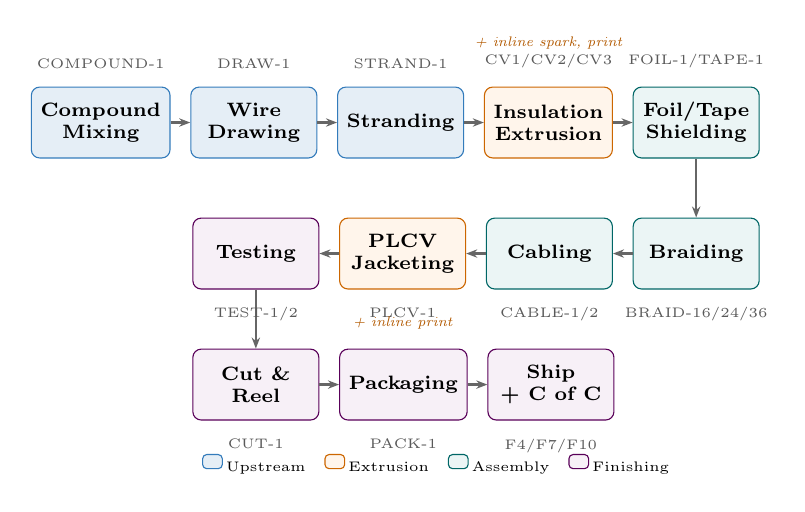
\begin{tikzpicture}[
    node distance=0.25cm and 0.25cm,
    % ── Category color styles ──
    upstream/.style={rectangle, draw=secblue!80, fill=secblue!10,
                     rounded corners=3pt, minimum width=1.6cm, minimum height=0.9cm,
                     align=center, font=\scriptsize\bfseries},
    extrusion/.style={rectangle, draw=orange!80!black, fill=orange!8,
                      rounded corners=3pt, minimum width=1.6cm, minimum height=0.9cm,
                      align=center, font=\scriptsize\bfseries},
    assembly/.style={rectangle, draw=teal!80!black, fill=teal!8,
                     rounded corners=3pt, minimum width=1.6cm, minimum height=0.9cm,
                     align=center, font=\scriptsize\bfseries},
    finishing/.style={rectangle, draw=violet!70!black, fill=violet!6,
                      rounded corners=3pt, minimum width=1.6cm, minimum height=0.9cm,
                      align=center, font=\scriptsize\bfseries},
    optional/.style={rectangle, draw=red!60!black, fill=red!5,
                     rounded corners=3pt, minimum width=1.35cm, minimum height=0.65cm,
                     align=center, font=\tiny\bfseries, dashed},
    ann/.style={font=\tiny, align=center, text=black!65},
    arr/.style={-{Stealth[length=4pt]}, thick, black!60},
    optarr/.style={-{Stealth[length=3pt]}, thin, red!50!black, dashed}
]
% ═══ Row 1: Upstream + Extrusion ═══
\node[upstream]  (comp)   {Compound\\Mixing};
\node[upstream,  right=of comp]   (draw)   {Wire\\Drawing};
\node[upstream,  right=of draw]   (strand) {Stranding};
\node[extrusion, right=of strand] (cv)     {Insulation\\Extrusion};
\node[assembly,  right=of cv]     (shield) {Foil/Tape\\Shielding};

% ═══ Row 2: Assembly + Jacketing ═══
\node[assembly,  below=0.75cm of shield] (braid) {Braiding};
\node[assembly,  left=of braid]          (cable) {Cabling};
\node[extrusion, left=of cable]          (plcv)  {PLCV\\Jacketing};
\node[finishing, left=of plcv]           (test)  {Testing};

% ═══ Row 3: Finishing ═══
\node[finishing, below=0.75cm of test] (cut)  {Cut \&\\Reel};
\node[finishing, right=of cut]         (pack) {Packaging};
\node[finishing, right=of pack]        (ship) {Ship\\+ C~of~C};

% ═══ Main-flow arrows ═══
\draw[arr] (comp) -- (draw);
\draw[arr] (draw) -- (strand);
\draw[arr] (strand) -- (cv);
\draw[arr] (cv) -- (shield);
\draw[arr] (shield) -- (braid);
\draw[arr] (braid) -- (cable);
\draw[arr] (cable) -- (plcv);
\draw[arr] (plcv) -- (test);
\draw[arr] (test) -- (cut);
\draw[arr] (cut) -- (pack);
\draw[arr] (pack) -- (ship);

% ═══ Work-center annotations ═══
\node[ann, above=3pt of comp]    {COMPOUND-1};
\node[ann, above=3pt of draw]    {DRAW-1};
\node[ann, above=3pt of strand]  {STRAND-1};
\node[ann, above=3pt of cv]      {CV1/CV2/CV3};
\node[ann, above=3pt of shield]  {FOIL-1/TAPE-1};
\node[ann, below=3pt of braid]   {BRAID-16/24/36};
\node[ann, below=3pt of cable]   {CABLE-1/2};
\node[ann, below=3pt of plcv]    {PLCV-1};
\node[ann, below=3pt of test]    {TEST-1/2};
\node[ann, below=3pt of cut]     {CUT-1};
\node[ann, below=3pt of pack]    {PACK-1};
\node[ann, below=3pt of ship]    {F4/F7/F10};

% ═══ Inline annotations (spark + print on extrusion nodes) ═══
\node[font=\tiny\itshape, text=orange!70!black, anchor=south]
  at ([yshift=0.35cm]cv.north) {+ inline spark, print};
\node[font=\tiny\itshape, text=orange!70!black, anchor=north]
  at ([yshift=-0.22cm]plcv.south) {+ inline print};

% ═══ Legend ═══
\node[anchor=north west, font=\tiny] at ([yshift=-0.3cm]cut.south west) {%
  \tikz[baseline=-0.5ex]{\fill[secblue!10,draw=secblue!80,rounded corners=1.5pt] (0,0) rectangle (0.25,0.18);}\,Upstream\quad
  \tikz[baseline=-0.5ex]{\fill[orange!8,draw=orange!80!black,rounded corners=1.5pt] (0,0) rectangle (0.25,0.18);}\,Extrusion\quad
  \tikz[baseline=-0.5ex]{\fill[teal!8,draw=teal!80!black,rounded corners=1.5pt] (0,0) rectangle (0.25,0.18);}\,Assembly\quad
  \tikz[baseline=-0.5ex]{\fill[violet!6,draw=violet!70!black,rounded corners=1.5pt] (0,0) rectangle (0.25,0.18);}\,Finishing
};

\end{tikzpicture}
\caption{SodhiCable production process flow (typical instrumentation cable routing).  Color indicates stage category.  Inline spark testing and printing/marking run continuously during insulation and jacketing extrusion.  Optional stations not shown: ARMOR-1 (armored MIL-DTL cable), CCCW-1 (corrugated copper welding for UL-2196), LPML-1 (LSOH jacketing), and DHT routing (PT-1 $\to$ NJ-EXT $\to$ PX-1).  Shipment requires F4-generated Certificate of Compliance.}
\label{fig:processflow}
\end{figure}

The typical routing begins at COMPOUND-1 (Banbury mixer for PVC, XLPE, or LSOH compounds), proceeds to DRAW-1 (wire drawing from 8\,mm rod to final gauge), then stranding on STRAND-1 (bunching or concentric lay to form multi-strand conductors; solid-conductor products skip this step), insulation extrusion on one of three CV lines selected by conductor size (CV2 for small gauges at 3{,}000\,ft/hr, CV1 for mid-range at 400\,ft/hr, CV3 for heavy gauges at 300\,ft/hr) with inline printing/marking (continuous footage marking, UL/CSA listing legend, and manufacturer identification are printed inline during both insulation and jacketing extrusion), foil or tape shielding (FOIL-1/TAPE-1), braiding (BRAID-16/-24/-36 depending on carrier count), cabling (CABLE-1/-2), jacketing on PLCV-1 (Pressurized Liquid Continuous Vulcanization), testing (spark test, DC resistance, and dimensional on TEST-1/-2), cutting (CUT-1), and final packaging (PACK-1).  Product-specific variations include armoring on ARMOR-1 for MIL-DTL power cables, CCCW-1 corrugated copper welding for UL-2196 fire-rated cable, and LPML-1 Large Poly Mold Line for LSOH shipboard jacketing.  The DHT process has a unique multi-site routing: PT-1 (pressure tubing extrusion) applies FEP insulation onto fiber, the resulting components ship to NJ-EXT where they are assembled into welded tube, and the assemblies return for PX-1 high-temperature encapsulation.  Lot genealogy (F10) traces material through every stage, and OEE (F11) is computed per work center per shift.


\subsection{Why All 11 MESA Functions Are Needed}

\begin{enumerate}[leftmargin=1.8em, itemsep=1pt]
\item \textbf{F1 --- Resource Allocation \& Status:} Assigns 26 work centers (compounding, drawing, stranding, CV insulation extrusion, braiders, cablers, PLCV, armoring, printing, testing, etc.) to work orders using an LP model that maximizes throughput while respecting line capability (gauge-based eligibility for CV1/CV2/CV3) and tooling constraints.
\item \textbf{F2 --- Operations Scheduling:} Sequences work orders across lines using SPT, EDD, or MILP to minimize total weighted tardiness and changeover scrap, accounting for setup-dependent product family transitions (e.g., compound color changes on CV lines).
\item \textbf{F3 --- Dispatching:} Releases scheduled jobs to the shop floor via a weighted priority dispatch rule that balances due-date urgency, customer priority (MIL-DTL Defense vs.\ Industrial), and changeover cost.
\item \textbf{F4 --- Document Control:} Version-controls Technical Methods (TM numbers), recipes, SOPs, and print legend specifications; generates Certificates of Compliance (C~of~C) and shipping test reports by aggregating F7 test data, F10 material traceability, and applicable spec revisions; ensures only the current approved recipe drives each production run.
\item \textbf{F5 --- Data Collection \& Acquisition:} Collects real-time sensor data (line speed, extruder temperature, spark-test voltage, environmental readings) and logs every production event with timestamps.
\item \textbf{F6 --- Labor Management:} Maintains a skill matrix for operator certifications (Operator, Setup, QA, Lead), solves an IP shift-rostering problem across $\approx$100 personnel, and tracks labor efficiency per shift.
\item \textbf{F7 --- Quality Management:} Monitors insulation/jacket OD and cut length on every extrusion line via $\bar{X}$-$R$ control charts, computes $C_{pk}$ per parameter per work center, and manages NCR$\to$CAPA workflows for spark-test failures and dimensional non-conformances.
\item \textbf{F8 --- Process Management:} Owns the ISA-88 recipe hierarchy for extrusion parameters (CV zone temperatures, PLCV vulcanization pressure, Banbury mix time) and detects sustained drift via CUSUM/EWMA.
\item \textbf{F9 --- Maintenance Management:} Schedules preventive maintenance on drawing dies, extrusion crossheads and tip/die assemblies, capstan pads, extruder screws, braider carriers, and PLCV salt-bath levels and seal quality using MTBF-based intervals; manages instrument calibration (laser gauges, spark electrodes, footage counters); and logs corrective actions for unplanned failures.
\item \textbf{F10 --- Product Tracking \& Genealogy:} Links every finished reel to its input copper lot, compound batch (from COMPOUND-1), and process conditions at every station, enabling sub-minute forward and backward recall traces.  Also enforces compound shelf-life expiration via FIFO lot selection and automatic quarantine.
\item \textbf{F11 --- Performance Analysis:} Computes OEE (Availability $\times$ Performance $\times$ Quality) per work center per shift and aggregates KPIs for the Tier~3 management review.
\end{enumerate}

\subsection{MESA-11 Summary Table}

\begin{table}[H]\centering\small
\caption{MESA-11 Function Summary --- SodhiCable}
\begin{tabularx}{\textwidth}{@{} l L{3.2cm} L{3.0cm} L{3.0cm} L{2.2cm} @{}}
\toprule
\textbf{Fn} & \textbf{Role at SodhiCable} & \textbf{Key Tables} & \textbf{Key Algorithm} & \textbf{Primary KPI} \\
\midrule
F1  & Assign lines \& dies to WOs & Resources, Work\-Orders, Routings & LP assignment & Utilization \% \\
F2  & Sequence jobs on lines & Work\-Orders, Schedule, Changeover\-Matrix & SPT / EDD / MILP & Total tardiness \\
F3  & Release jobs to floor & dispatch\_queue, dispatch\_log & Weighted priority dispatch & Queue time \\
F4  & Version-control recipes & Recipes, Recipe\-Parameters, Documents & Version workflow & Doc currency \\
F5  & Sensor \& event logging & Process\-Data\-Live, Spark\-Test\-Log & Threshold alarm & Data capture \% \\
F6  & Staff skills \& rostering & Personnel, Personnel\-Certs, Shift\-Handoff & IP rostering & Labor efficiency \\
F7  & SPC \& non-conformance & SPC\-Readings, Test\-Results, NCR & $\bar{X}$-$R$, $C_{pk}$ & FPY / RTFT \\
F8  & Recipe execution \& control & Recipe\-Params, Process\-Deviations, Hold\-Release & PID / CUSUM / EWMA & Deviation rate \\
F9  & PM \& corrective maint. & Equipment, Maintenance, Downtime\-Log & MTBF-based PM & MTBF (hrs) \\
F10 & Lot genealogy \& recall & Lot\-Tracking, Reel\-Inventory, Inventory & Recursive CTE trace & Recall time \\
F11 & OEE \& shift reporting & KPIs, Scrap\-Log, Shift\-Reports & OEE = $A \times P \times Q$ & OEE \% \\
\bottomrule
\end{tabularx}
\end{table}


\subsection{Functions Beyond the MESA-11 Framework}

The MESA-11 model (1997) provides a comprehensive functional specification but predates IoT, cloud computing, and AI. The SodhiCable prototype extends beyond the original 11 functions with 20 additional capabilities:

\begin{enumerate}[leftmargin=2em, itemsep=1pt]
\item \textbf{Discrete Event Simulation (DES):} 8-stage factory model with 5 dispatch rules (FIFO, SPT, EDD, WSPT, Campaign), M/M/1 and M/M/c queueing analytics, and what-if scenario analysis.
\item \textbf{Material Requirements Planning (MRP):} Multi-level BOM explosion with 7 lot-sizing methods (L4L, EOQ, POQ, FOQ, Silver-Meal, Wagner-Whitin, EPQ).
\item \textbf{AI/ML Intelligence Layer:} Claude API natural-language-to-SQL queries, z-score anomaly detection on process data, MTBF-based failure probability prediction, quality risk correlation, and a rules-based recommendation engine (see Section~\ref{sec:ai}).
\item \textbf{ISA-95 SCADA Visualization:} Level 3 $\to$ Level 2 $\to$ Level 1 drill-down with energy monitoring, PLC/controller simulation, and spark test results.
\item \textbf{OPC-UA Tag Simulator:} Background thread generating continuous sensor readings at configurable intervals, demonstrating how the MES connects to real PLCs.
\item \textbf{Predictive Maintenance:} Exponential failure model $P(\text{fail}) = 1 - e^{-t/\text{MTBF}}$ with cost-of-delay analysis.
\item \textbf{Supply Chain Risk Analysis:} Material coverage heat map, single-source supplier detection, lead-time variability scoring.
\item \textbf{Bottleneck Analysis:} Kingman's G/G/c approximation with shifting bottleneck identification and capacity what-if scenarios.
\item \textbf{Energy Management:} kWh tracking per work center (4{,}800 energy readings), kWh/KFT efficiency metric for extrusion lines, lb/hr for compounding.
\item \textbf{Visual Genealogy:} Interactive tree/graph toggle for lot traceability with layered node rendering by tier.
\item \textbf{Recipe Version Comparison:} Side-by-side parameter diff between recipe versions with change highlighting.
\item \textbf{Global Search \& Notifications:} Cross-table search across WOs, products, equipment, personnel, and lots. Notification center aggregating alarms, overdue PMs, late WOs, and expiring certifications.
\item \textbf{System Meta-Metrics:} Dashboard monitoring the MES itself --- endpoint count, DB size, table statistics, data freshness.
\item \textbf{Shift Report Generation:} Auto-calculate OEE ($A \times P \times Q$) from actual downtime, output, and scrap data.
\item \textbf{ERP Level 4 Simulation:} Complete ISA-95 Level 4 implementation including purchase order management, goods receipt inspection, customer invoicing, shipment tracking, and demand forecasting. The ERP simulator generates ISA-95 B2MML-style messages crossing the L3$\leftrightarrow$L4 boundary.
\item \textbf{Certificate of Compliance Generation:} Automated C of C per work order aggregating test results, lot genealogy (backward trace to raw material), and applicable specification compliance (MIL-DTL, UL, API).
\item \textbf{Splice Zone Detection:} Identifies output lots with multiple distinct input lots, indicating conductor payoff splices. Critical for MIL-SPEC traceability where splice zones require customer acceptance.
\item \textbf{S\&OP Demand Forecasting:} Simple moving average and trend-based demand forecasting engine feeding the MRP planned order generation.
\item \textbf{SSE Real-Time Streaming:} Server-Sent Events endpoints for continuous process data and alarm streaming to browser clients, enabling real-time dashboards without polling.
\item \textbf{Weibull Remaining Useful Life:} Equipment failure modeling using the Weibull CDF for condition-based PM scheduling with interactive Chart.js visualizations.
\end{enumerate}

MESA International later expanded to the Strategic Initiatives Model (2004+) and Smart Manufacturing Model, recognizing that modern MES/MOM must address Lean Manufacturing, Asset Performance Management, and Real-Time Enterprise integration --- capabilities that the SodhiCable prototype already incorporates.


\subsection{Cross-Function Data Flow Map}

The 11 MESA functions do not operate in isolation --- each function produces data consumed by others.  The primary data flows at SodhiCable are:

\begin{itemize}[leftmargin=1.8em, itemsep=1pt]
\item \textbf{Planning chain:} F1 (resource assignment) $\to$ F2 (scheduling) $\to$ F3 (dispatching) $\to$ shop floor execution.  F1 reads capacity from \tfield{work\_centers} (26 WCs) and demand from \tfield{work\_orders}; F2 sequences using \tfield{routings} and passes to F3's \tfield{dispatch\_queue}.
\item \textbf{Execution chain:} F5 (data collection) feeds F8 (process monitoring) and F7 (quality).  Sensor data flows through \tfield{process\_data\_live} to F8's PID/CUSUM/EWMA algorithms; inspection results flow through \tfield{spc\_readings} to F7's control charts.
\item \textbf{Quality chain:} F7 (quality alarm) $\to$ F10 (lot quarantine) $\to$ F10 (forward trace) $\to$ F4 (CAPA documentation).  An out-of-control signal sets \tfield{spc\_readings.status}~=~`OOC', triggering an NCR in \tfield{ncr}, quarantining the lot in \tfield{inventory}, and tracing affected lots via \tfield{lot\_tracking}.
\item \textbf{Maintenance chain:} F9 (PM scheduling / corrective maintenance) $\to$ F1 (capacity reduction) $\to$ F2 (reschedule).  \tfield{equipment.status}~=~`Down' removes the WC from F1's 26-machine capacity pool.
\item \textbf{Reporting chain:} F11 aggregates from all functions --- \tfield{downtime\_log} (F9), \tfield{scrap\_log} (F7), \tfield{dispatch\_log} (F3), \tfield{shift\_handoff} (F6) --- to compute OEE and KPIs in \tfield{shift\_reports}.
\item \textbf{Labor chain:} F6 (certifications) $\to$ F3 (dispatch qualification check) $\to$ F1 (labor assignment).  \tfield{personnel\_certs} (Operator, Setup, QA, Lead) gates which operators may run which lines.
\item \textbf{Recipe chain:} F4 (document control) $\to$ F8 (recipe setpoints) $\to$ F5 (monitoring against limits).  \tfield{recipe\_parameters} defines setpoints (CV zone temps, PLCV pressure, Banbury mix time) that F8 monitors and F5 collects data against.
\item \textbf{Compound chain:} F10 (lot tracking) $\to$ COMPOUND-1 (batch identity) $\to$ CV/PLCV (compound consumption) $\to$ F10 (reel genealogy).  Every compound batch from the Banbury mixer is traced through all downstream stations to finished reels.
\end{itemize}


\subsection{Assumptions \& Design Constraints}

The following assumptions bound the scope of this MES design:

\begin{enumerate}[leftmargin=1.8em, itemsep=2pt]
\item \textbf{Single-site scope.}  This design covers the primary SodhiCable manufacturing facility.  External processing at the NJ facility (NJ-EXT, welded-tube DHT assemblies) is modeled as an outbound/inbound material transfer in \tfield{lot\_tracking}.  The ERP interface is modeled as a flat-file or API exchange at the \tfield{sales\_orders} boundary.
\item \textbf{SQLite as prototype DBMS.}  All tables reside in a single \texttt{sodhicable\_mes.db} file.  A production deployment would migrate to PostgreSQL or SQL Server for concurrent multi-user access, but the relational schema and FK constraints are identical.
\item \textbf{Deterministic processing times.}  LP and scheduling algorithms (F1, F2) use mean processing rates from historical data.  Stochastic variability is captured post-hoc through OEE (F11) and Kingman's formula rather than embedded in the optimization models.
\item \textbf{100\% spark testing.}  Every reel undergoes a full-length spark test per customer specification; sampling plans apply only to dimensional SPC (F7).
\item \textbf{Three-shift, 24/7 operation.}  The rostering IP (F6) assumes three 8-hour shifts with no planned overtime.  OSHA rest-period and maximum-hours constraints are hard constraints in the model.
\item \textbf{Recipe hierarchy follows ISA-88.}  General $\to$ Site $\to$ Master $\to$ Control recipe levels are implemented; the prototype populates Master and Control levels only.
\item \textbf{Sensor data granularity.}  \tfield{process\_data\_live} stores one reading per sensor per scan interval (configurable, default 5~seconds).  The prototype seeds representative data at 1-minute intervals to keep database size manageable.
\item \textbf{MRP module (prototype scope).}  The prototype now includes an MRP module with multi-level BOM explosion and 7 lot-sizing methods (L4L, EOQ, POQ, FOQ, Silver-Meal, Wagner-Whitin, EPQ).  In a production deployment, MRP would be handled by the upstream ERP with bidirectional sync; the prototype MRP demonstrates the algorithm and generates planned orders in \tfield{mrp\_planned\_orders} but does not generate purchase orders.
\item \textbf{Canonical units.}  Length-of-cable quantities are stored in feet (ft) at the transactional level (\tfield{lot\_tracking.qty\_consumed}, \tfield{scrap\_log.quantity\_ft}); work-order sizes are in thousand-feet (kft); line rates are in ft/hr; and insulation-resistance is reported per 1000~ft.  Unit conversions are centralised in \tfield{unit\_conversions}.
\end{enumerate}

These constraints ensure the prototype remains tractable for a semester project while preserving the structural fidelity needed to demonstrate all 11 MESA functions end-to-end.

\textbf{Known Limitations \& Future Work.}  The prototype now includes an OPC-UA tag simulator with background-thread sensor generation, but does not yet connect to real PLCs --- \tfield{process\_data\_live} is populated by the simulated sensor writer rather than live field devices.  Remaining limitations: (i)~NJ-EXT integration --- the external welded-tube facility is tracked as a material transfer but not optimized jointly with on-site scheduling; (ii)~stochastic scheduling --- F2 uses mean processing times, and variability is handled post-hoc in F11 via Kingman's approximation; (iii)~full MES--ERP bidirectional sync --- work-order releases are read once per scheduling cycle rather than streamed.  These are scoped for a Phase~2 production build.


%======================================================================
\section{Database Design --- Table Specifications}\label{sec:schema}
%======================================================================

The SodhiCable MES uses a single SQLite database (\texttt{sodhicable\_mes.db}).  Each MESA function is presented below with its business role, table specifications, key algorithm, and integration notes.

Figure~\ref{fig:erdiagram} shows the 78-table schema clustered by MESA function, highlighting the principal foreign-key relationships that carry information between functions.  Reference tables (\tfield{products}, \tfield{work\_centers}, \tfield{personnel}, \tfield{customers}, \tfield{plants}) are shared across functions and shown in the central hub.

\begin{figure}[H]\centering
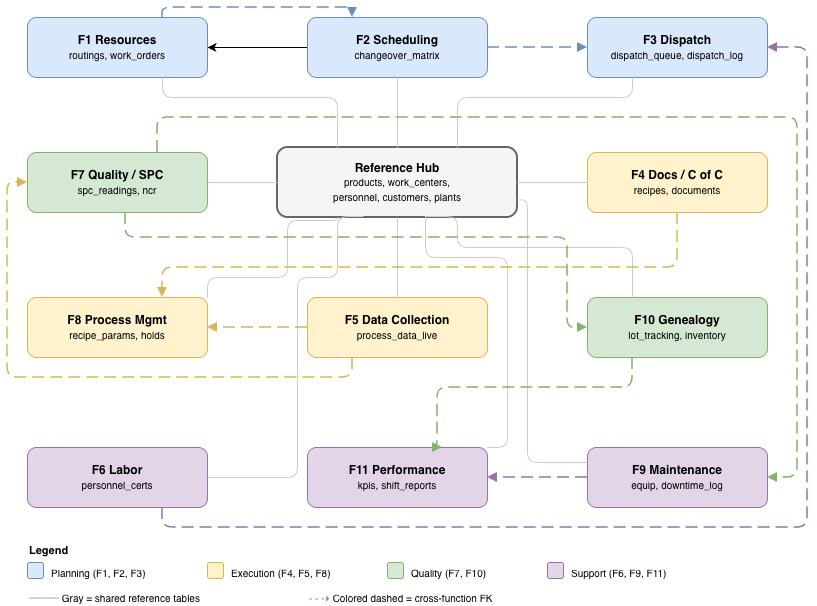
\includegraphics[width=\textwidth]{SodhiCable_ER_Diagram.drawio.png}
\caption{SodhiCable MES 78-table schema clustered by MESA function.  Color indicates function group: \textcolor{secblue}{\textbf{Planning}} (F1$\to$F2$\to$F3 schedule chain), \textcolor{orange!80!black}{\textbf{Execution}} (F4 recipes/C\,of\,C, F5 data, F8 process control), \textcolor{teal!80!black}{\textbf{Quality}} (F7 SPC/NCR, F10 genealogy/traceability), and \textcolor{violet!70!black}{\textbf{Support}} (F6 labor, F9 maintenance, F11 KPIs).  All functions read from the central Reference Hub (shared dimension tables).  Colored dashed arrows show principal cross-function FK relationships.}
\label{fig:erdiagram}
\end{figure}


%----------------------------------------------------------------------
\subsection{F1 --- Resource Allocation \& Status}
%----------------------------------------------------------------------

\textbf{Business Role.}
F1 tracks every physical production resource --- 26 work centers spanning compounding, drawing, stranding, CV extrusion, braiding, cabling, PLCV vulcanization, armoring, printing/marking, testing, cutting, and packaging --- and assigns them to work orders.  When a new set of work orders is released, F1 solves an LP to maximize total throughput subject to line capability (product--WC eligibility from \tfield{routings}) and capacity constraints.

\subsubsection*{Table: work\_centers}
\begin{table}[H]\centering\small
\begin{tabular}{@{} l l l L{6cm} @{}}
\toprule
\textbf{Field} & \textbf{Type} & \textbf{Role} & \textbf{Description} \\
\midrule
wc\_id          & TEXT    & PK  & Unique work-center code (e.g.\ CV1, DRAW-1) \\
name            & TEXT    &     & Human-readable name \\
equipment\_type & TEXT    &     & Compounding, Drawing, Stranding, Insulation Extrusion, Jacketing, Braiding, Cabling, Printing, Testing, Packaging \\
capacity\_hrs\_per\_week & REAL & & Available hours per week \\
utilization\_target & REAL &   & Target utilization (default 0.80) \\
setup\_time\_min & REAL   &     & Default changeover time (minutes) \\
cost\_per\_hr   & REAL    &     & Hourly operating cost (\$) \\
manning         & REAL    &     & Operators required per shift \\
capacity\_ft\_per\_hr & REAL & & Throughput rate (ft/hr) \\
\bottomrule
\end{tabular}
\end{table}

\subsubsection*{Table: work\_orders}
\begin{table}[H]\centering\small
\begin{tabular}{@{} l l l L{6cm} @{}}
\toprule
\textbf{Field} & \textbf{Type} & \textbf{Role} & \textbf{Description} \\
\midrule
wo\_id       & TEXT     & PK  & Work-order identifier \\
product\_id  & TEXT     & FK$\to$products & Product to manufacture \\
business\_unit & TEXT   &     & Defense, Infrastructure, Industrial, OilGas \\
order\_qty\_kft & REAL  &     & Order quantity (thousands of feet) \\
priority     & INTEGER  &     & 1 (highest) to 5 (lowest) \\
due\_date    & TEXT     &     & Customer due date \\
created\_date & TEXT    &     & Order creation timestamp \\
status       & TEXT     &     & Pending $\mid$ Released $\mid$ In-Progress $\mid$ Complete \\
\bottomrule
\end{tabular}
\end{table}

\subsubsection*{Table: routings}
\begin{table}[H]\centering\small
\begin{tabular}{@{} l l l L{6cm} @{}}
\toprule
\textbf{Field} & \textbf{Type} & \textbf{Role} & \textbf{Description} \\
\midrule
routing\_id   & INTEGER & PK  & Auto-increment row ID \\
product\_id   & TEXT    & FK$\to$products & Product this routing serves \\
sequence\_num & INTEGER &     & Operation step (10, 20, 30\ldots) \\
wc\_id        & TEXT    & FK$\to$work\_centers & Work center for this step \\
process\_time\_min\_per\_100ft & REAL & & Standard processing rate \\
\bottomrule
\end{tabular}
\end{table}

\subsubsection*{Key Algorithm --- LP Resource Assignment (Week 3 / Week 6)}

\begin{eqbox}[F1 --- LP Resource Assignment]
\textbf{Objective:} Assign $n$ work orders to $m$ work centers to maximize total throughput:
\[
\max \sum_{i=1}^{n}\sum_{j=1}^{m} r_{ij}\, x_{ij}
\]
\textbf{Decision variables:} $x_{ij} \in \{0,1\}$ --- 1 if WO $i$ is assigned to WC $j$.

\textbf{Constraints:}
\begin{align}
\sum_{j=1}^{m} x_{ij} &= 1 \quad \forall\, i & &\text{(each WO assigned exactly once)} \\
\sum_{i=1}^{n} t_{ij}\, x_{ij} &\leq C_j \quad \forall\, j & &\text{(capacity limit per WC)} \\
x_{ij} &= 0 \quad \text{if WC } j \text{ lacks capability for product } i
\end{align}
\textbf{Parameters:} $r_{ij}$ = revenue-per-kft (from \tfield{products}); $t_{ij}$ = processing time (from \tfield{routings.process\_time\_min\_per\_100ft}); $C_j$ = available capacity (from \tfield{work\_centers.capacity\_hrs\_per\_week}).  With 26 work centers and 33+ products, the LP has $\approx$858 decision variables.
\end{eqbox}

\textit{Parameters from the Week~3 capacity model.}
Rated throughputs from \tfield{work\_centers.\allowbreak capacity\_ft\_per\_hr}:
CV2 = 3{,}000\,ft/hr (small-gauge, 75\,min setup),
CV1 = 400\,ft/hr (mid-gauge, 90\,min setup),
CV3 = 300\,ft/hr (heavy-gauge, 75\,min setup),
CABLE-1 = 40\,hrs/wk assembly,
DRAW-1 = 5{,}000\,ft/hr.
Dual prices from the Week~3 LP identified copper rod as the binding resource (shadow price ${\approx}\$4.80$/ft), confirming throughput is gated by upstream copper supply rather than CV line capacity.

\textbf{Integration Notes.}
F1 receives released work orders from F2 (reading \tfield{work\_orders.\allowbreak status}\,=\,`Released') and passes the assigned work center to F3 via \tfield{dispatch\_queue.\allowbreak wc\_id}.  F1 reads \tfield{work\_centers.\allowbreak capacity\_hrs\_per\_week} and \tfield{routings.\allowbreak process\_time\_min\_per\_100ft} to compute capacity loading.  F9 reduces available capacity by setting \tfield{equipment.status}\,=\,`Down' during maintenance events.

%----------------------------------------------------------------------
\subsection{F2 --- Operations Scheduling}
%----------------------------------------------------------------------

\textbf{Business Role.}
F2 sequences released work orders across production lines to minimize total weighted tardiness and changeover waste, accounting for setup-dependent transitions between product families.  In wire-and-cable manufacturing, changeover cost is dominated by compound purging on CV extrusion lines (switching insulation material requires flushing the screw and barrel) and by die changes on the drawing machines, so the scheduler groups jobs by product family (A, B, C, D, I, M, R, S, U) to minimize these transitions.  The \tfield{changeover\_matrix} table stores family-to-family setup times and scrap costs, which the scheduling algorithm reads when evaluating candidate sequences.

\subsubsection*{Table: products}
\begin{table}[H]\centering\small
\begin{tabular}{@{} l l l L{6cm} @{}}
\toprule
\textbf{Field} & \textbf{Type} & \textbf{Role} & \textbf{Description} \\
\midrule
product\_id      & TEXT & PK  & Unique product code \\
name             & TEXT &     & Product description \\
family           & TEXT &     & Product family (A=Instrumentation, B=Control/Power, C=DHT, D=DHT FlatPack, I=Insulated Conductor, M=Medium Voltage, R=Building Wire, S=Shipboard/LSOH, U=UL-2196) \\
revenue\_per\_kft & REAL &    & Revenue rate (\$/kft) \\
cost\_per\_kft   & REAL &     & Variable production cost (\$/kft) \\
max\_order\_qty\_kft & REAL & & Maximum single-order quantity \\
\bottomrule
\end{tabular}
\end{table}

\subsubsection*{Table: changeover\_matrix}
\begin{table}[H]\centering\small
\begin{tabular}{@{} l l l L{6cm} @{}}
\toprule
\textbf{Field} & \textbf{Type} & \textbf{Role} & \textbf{Description} \\
\midrule
from\_product    & TEXT & PK  & Product code of preceding job \\
to\_product      & TEXT & PK  & Product code of following job \\
setup\_minutes   & REAL &     & Changeover duration (min) \\
scrap\_ft        & REAL &     & Expected scrap footage during changeover \\
compound\_change & INTEGER &  & 1 if compound color change required \\
\bottomrule
\end{tabular}
\end{table}

\subsubsection*{Table: schedule}
\begin{table}[H]\centering\small
\begin{tabular}{@{} l l l L{5.5cm} @{}}
\toprule
\textbf{Field} & \textbf{Type} & \textbf{Role} & \textbf{Description} \\
\midrule
schedule\_id     & INTEGER & PK  & Auto-increment ID \\
wo\_id           & TEXT    & FK$\to$work\_orders & Scheduled work order \\
wc\_id           & TEXT    & FK$\to$work\_centers & Assigned work center \\
sequence\_pos    & INTEGER &     & Position in the sequence (1, 2, \ldots) \\
planned\_start   & TEXT    &     & Planned start timestamp \\
planned\_end     & TEXT    &     & Planned end timestamp \\
setup\_minutes   & REAL    &     & Setup time before this job (from changeover matrix) \\
status           & TEXT    &     & Planned $\mid$ In-Progress $\mid$ Completed \\
\bottomrule
\end{tabular}
\end{table}

\subsubsection*{Key Algorithm --- SPT / EDD / MILP Scheduling (Week 4 / Week 6)}

\begin{eqbox}[F2 --- Scheduling Dispatch Rules]
\textbf{SPT:} sequence by non-decreasing processing time $p_{[1]} \leq p_{[2]} \leq \cdots \leq p_{[n]}$; minimizes mean flow time $\bar{F}$.\\
\textbf{EDD:} sequence by non-decreasing due date $d_{[1]} \leq d_{[2]} \leq \cdots \leq d_{[n]}$; minimizes maximum lateness $L_{\max}$.\\
\textbf{WSPT:} sequence by non-increasing $w_i / p_i$; minimizes $\sum w_i C_i$.
\end{eqbox}

\begin{eqbox}[F2 --- MILP Total Weighted Tardiness (exact, $n \leq 20$)]
\textbf{Sets:} $\mathcal{J} = \{1, \ldots, n\}$ jobs;\; $\mathcal{M} = \{1, \ldots, m\}$ work centers.

\textbf{Decision variables:} $x_{ij} \in \{0,1\}$ (job-to-WC assignment);\; $y_{ik} \in \{0,1\}$ (precedence);\; $C_i \geq 0$ (completion time);\; $T_i \geq 0$ (tardiness, $T_i = \max(0, C_i - d_i)$).

\textbf{Objective:} Minimize total weighted tardiness:
\[
\min \sum_{i \in \mathcal{J}} w_i \, T_i
\]
\textbf{Constraints:}
\begin{alignat}{2}
\sum_{j \in \mathcal{M}} x_{ij} &= 1 &\quad& \forall\, i \in \mathcal{J} \\
C_i &\geq C_k + s_{ki} + p_{ij} - M(1 - y_{ki}) &\quad& \forall\, i,k,j \\
T_i &\geq C_i - d_i &\quad& \forall\, i \in \mathcal{J} \\
x_{ij} &\leq a_{ij} &\quad& \forall\, i,j \;\text{(line capability)}
\end{alignat}
\textbf{Parameters:} $p_{ij}$ = processing time (\tfield{routings});\; $s_{ki}$ = setup time (\tfield{changeover\_matrix});\; $d_i$ = due date;\; $w_i$ = priority weight;\; $a_{ij}$ = line eligibility;\; $M$ = big-$M$ constant.
\end{eqbox}

\textit{Typical values:} $w_i = 3$ for shipboard/UL-2196 (S, U); $w_i = 2$ for MV and control/power (M, B); $w_i = 1$ for building wire and instrumentation (R, A).  Setup times $s_{ki}$: 15~min (same family) to 90~min (compound color change).  For $n > 20$, the solver is seeded with WSPT and terminated at a 2\% gap.

\textbf{Integration Notes.}
F2 receives assigned work orders from F1 (reading \tfield{work\_orders.wo\_id} where \tfield{status}~=~`Released') and writes the sequenced schedule to \tfield{schedule} with computed \tfield{planned\_start} and \tfield{planned\_end}, then populates F3's \tfield{dispatch\_queue} with \tfield{priority\_score}.  Setup times from \tfield{changeover\_matrix.setup\_minutes} are summed into F11's OEE Performance denominator via \tfield{downtime\_log.category}~=~`Setup'.  When F9 takes a line down for maintenance (\tfield{equipment.status}~=~`Down'), F2 reschedules affected jobs by re-solving the MILP with the reduced machine set.

%----------------------------------------------------------------------
\subsection{F3 --- Dispatching}
%----------------------------------------------------------------------

\textbf{Business Role.}
F3 releases scheduled jobs to the shop floor in real time, maintaining a prioritized dispatch queue per work center.  When an operator finishes a job, F3 selects the next job from the queue based on a weighted priority score that balances due-date urgency, customer importance, and changeover cost.

\subsubsection*{Table: dispatch\_queue}
\begin{table}[H]\centering\small
\begin{tabular}{@{} l l l L{5.5cm} @{}}
\toprule
\textbf{Field} & \textbf{Type} & \textbf{Role} & \textbf{Description} \\
\midrule
queue\_id      & INTEGER & PK  & Auto-increment ID \\
wo\_id         & TEXT    & FK$\to$work\_orders & Work order awaiting dispatch \\
wc\_id         & TEXT    & FK$\to$work\_centers & Target work center \\
priority\_score & REAL   &     & Computed dispatch score $S_i$ \\
queue\_position & INTEGER &    & Rank in queue (1 = next to run) \\
enqueued\_at   & TEXT    &     & Timestamp job entered queue \\
status         & TEXT    &     & Waiting $\mid$ Dispatched $\mid$ Cancelled \\
\bottomrule
\end{tabular}
\end{table}

\subsubsection*{Table: dispatch\_log}
\begin{table}[H]\centering\small
\begin{tabular}{@{} l l l L{5.5cm} @{}}
\toprule
\textbf{Field} & \textbf{Type} & \textbf{Role} & \textbf{Description} \\
\midrule
log\_id         & INTEGER & PK  & Auto-increment ID \\
wo\_id          & TEXT    & FK$\to$work\_orders & Dispatched work order \\
wc\_id          & TEXT    & FK$\to$work\_centers & Work center job was released to \\
operator\_id    & TEXT    & FK$\to$personnel & Operator who received the job \\
dispatch\_time  & TEXT    &     & Timestamp of dispatch \\
completion\_time & TEXT   &     & Timestamp job completed (null if in progress) \\
priority\_score & REAL    &     & Score at time of dispatch (for audit) \\
\bottomrule
\end{tabular}
\end{table}

\subsubsection*{Key Algorithm --- Weighted Priority Dispatch (Week 5)}

\begin{eqbox}[F3 --- Weighted Priority Dispatch]
\textbf{Objective:} Select job $i^*$ from queue $Q_j$ that maximizes the dispatch score:
\[
i^* = \arg\max_{i \in Q_j} S_i, \qquad S_i = w_1 \cdot \frac{1}{d_i - t} \;+\; w_2 \cdot P_i \;+\; w_3 \cdot \frac{1}{s_{ij}+1}
\]
\textbf{Decision variable:} $x_i \in \{0,1\}$ --- 1 if job $i$ dispatched next on WC $j$.

\textbf{Constraints:}
\begin{alignat}{2}
\sum_{i \in Q_j} x_i &= 1 &\quad& \text{(one job per dispatch cycle)} \\
x_i &= 0 &\quad& \text{if operator lacks cert for product } i \;\text{(F6 check)}
\end{alignat}
\textbf{Parameters:} $d_i$ = due date; $t$ = current time; $P_i$ = customer priority (1--5); $s_{ij}$ = changeover time (\tfield{changeover\_matrix}); weights $w_1 = 0.4$, $w_2 = 0.4$, $w_3 = 0.2$.
\end{eqbox}

\textbf{Integration Notes.}
F3 consumes the schedule from F2 (reading \tfield{work\_orders.status}~=~`Released') and checks operator qualification via F6 (\tfield{personnel\_certs.certification\_type} matched against the product's required cert).  Each dispatch event writes to \tfield{dispatch\_log.dispatch\_time}, which F11 reads to compute schedule adherence KPIs.

\textbf{Lot-Sizing Policy (Week 7 commitments).}  Work-order quantities delivered to F3 follow a three-tier policy keyed to inventory class: \textbf{FOQ (fixed-order quantity)} is used for L1 finished-reel SKUs where reel length is standardised (e.g., 1000\,ft or 2500\,ft reels of building wire); \textbf{EOQ} is used for L2 intermediate stocks such as drawn copper and jacketed cores where holding and setup costs are balanced analytically ($Q^* = \sqrt{2DS/h}$); and \textbf{dynamic (Wagner--Whitin / period-balancing) lot-sizing} is used for L0 make-to-order MIL-DTL and UL-2196 jobs where demand is lumpy and customer-specific.  The resulting lot sizes populate \tfield{work\_orders.quantity\_ft} and drive the scheduling horizon consumed by F2.

%----------------------------------------------------------------------
\subsection{F4 --- Document Control}
%----------------------------------------------------------------------

\textbf{Business Role.}
F4 version-controls all Technical Methods (TMs), recipes, and SOPs.  Every extrusion, compounding, or cabling run must reference the current approved recipe revision (e.g., TM-2001 Rev~C for CV1 silicone insulation); expired revisions are locked.  F4 also governs the \emph{print legend specification} for each product --- the continuous text printed or embossed onto the cable surface inline during insulation and jacketing extrusion.  The legend includes the UL/CSA listing mark, manufacturer name, product catalog number, voltage rating, temperature rating, and sequential footage marking.  The correct legend format is stored per product in \tfield{documents} and verified by the operator at line startup; an incorrect print legend is a non-conformance requiring reel quarantine.

\textbf{Certificates of Compliance and Shipping Documentation.}
No reel ships without a Certificate of Compliance (C~of~C) certifying the product meets the applicable specification.  The C~of~C is the convergence point of F4, F7, and F10: F7's \tfield{test\_results} supplies the test data (spark, DC resistance, insulation resistance, dimensional, tensile), F10's \tfield{lot\_tracking} provides material traceability linking every reel to its input copper lot and compound batch, and F4's \tfield{documents} identifies the governing spec revision (UL, MIL-DTL, or customer-specific).  For standard commercial shipments, the C~of~C contains a summary certification with key test values.  Defense and shipboard customers (MIL-DTL-24643/24640) require a heavier documentation package: full test reports for every reel, raw-material mill certifications traced through F10 genealogy, and in some cases witness-test documentation signed by the customer's quality representative.  The C~of~C document is generated as a \tfield{documents} record with \tfield{doc\_type}\,=\,`Certificate' linked to the shipping work order, and archived for the retention period required by the applicable standard.

\subsubsection*{Table: recipes}
\begin{table}[H]\centering\small
\begin{tabular}{@{} l l l L{5.5cm} @{}}
\toprule
\textbf{Field} & \textbf{Type} & \textbf{Role} & \textbf{Description} \\
\midrule
recipe\_id      & INTEGER & PK  & Auto-increment ID \\
recipe\_code    & TEXT    & UQ  & Recipe identifier (e.g.\ REC-CV1-001) \\
description     & TEXT    &     & Recipe purpose / title \\
product\_id     & TEXT    & FK$\to$products & Product this recipe serves \\
work\_center\_id & TEXT   & FK$\to$work\_centers & Target work center \\
tm\_number      & TEXT    &     & Technical Method document number \\
tm\_revision    & TEXT    &     & Current TM revision (e.g.\ Rev C) \\
version         & INTEGER &     & Recipe version (auto-increment on change) \\
status          & TEXT    &     & Approved $\mid$ Draft $\mid$ Obsolete \\
approved\_by    & TEXT    &     & Approver's employee code \\
\bottomrule
\end{tabular}
\end{table}

\subsubsection*{Table: documents}
\begin{table}[H]\centering\small
\begin{tabular}{@{} l l l L{5.5cm} @{}}
\toprule
\textbf{Field} & \textbf{Type} & \textbf{Role} & \textbf{Description} \\
\midrule
doc\_id       & INTEGER & PK  & Auto-increment ID \\
wo\_id        & TEXT    & FK$\to$work\_orders & Associated work order (nullable) \\
doc\_type     & TEXT    &     & SOP, TM, Drawing, Certificate \\
doc\_name     & TEXT    &     & Document title \\
file\_path    & TEXT    &     & Storage path \\
created\_date & TEXT    &     & Creation timestamp \\
version       & TEXT    &     & Document version string \\
\bottomrule
\end{tabular}
\end{table}

\subsubsection*{Table: recipe\_ingredients}
\begin{table}[H]\centering\small
\begin{tabular}{@{} l l l L{5.0cm} @{}}
\toprule
\textbf{Field} & \textbf{Type} & \textbf{Role} & \textbf{Description} \\
\midrule
ingredient\_id & INTEGER & PK  & Auto-increment ID \\
recipe\_id     & INTEGER & FK$\to$recipes & Parent recipe \\
material\_id   & TEXT    & FK$\to$materials & Raw material / compound used \\
qty\_per\_kft   & REAL   &     & Quantity consumed per 1\,000\,ft of output \\
uom           & TEXT    &     & Unit of measure (LB, KG, GAL) \\
scrap\_allowance & REAL  &     & Expected scrap factor (e.g.\ 0.03 = 3\%) \\
\bottomrule
\end{tabular}
\end{table}

\subsubsection*{Key Algorithm --- Version Control Workflow \& Document Currency (Week 2)}

\textbf{State machine:} \texttt{Draft} $\xrightarrow{\text{review}}$ \texttt{Approved} $\xrightarrow{\text{supersede}}$ \texttt{Obsolete}.  Only recipes with \tfield{status}~=~`Approved' may be referenced by active work orders.  Each revision increments \tfield{version} and logs the change to \tfield{audit\_trail}.

\textbf{Document currency metric:}
\[
\text{Currency} = \frac{|\{d \in D : d.\text{status} = \texttt{Approved} \wedge d.\text{version} = \max(\text{version})\}|}{|D|}
\]
where $D$ is the set of all active documents and recipes.  Target: Currency $\geq 0.95$ (at most 5\% of active documents pending revision).  This KPI is computed weekly and written to \tfield{kpis.kpi\_name}~=~`Doc\_Currency'.

\textbf{Integration Notes.}
F4 supplies setpoints to F8 via \tfield{recipe\_parameters.parameter\_value}, \tfield{lower\_limit}, and \tfield{upper\_limit} for each recipe step.  F4 also feeds F10 through \tfield{recipe\_ingredients.material\_id}, linking each recipe to its bill of materials for genealogy tracing.  F7 reads \tfield{recipes.status} to confirm only `Approved' recipes are active before evaluating quality results.  Every revision change is logged to \tfield{audit\_trail.action}~=~`recipe\_update' with \tfield{changes} recording old vs.\ new values.

%----------------------------------------------------------------------
\subsection{F5 --- Data Collection \& Acquisition}
%----------------------------------------------------------------------

\textbf{Business Role.}
F5 is the data backbone --- it captures real-time sensor readings from extrusion lines (temperature, pressure, line speed) and spark-test results, feeding every other function.

\subsubsection*{Table: process\_data\_live}
\begin{table}[H]\centering\small
\begin{tabular}{@{} l l l L{6cm} @{}}
\toprule
\textbf{Field} & \textbf{Type} & \textbf{Role} & \textbf{Description} \\
\midrule
reading\_id & INTEGER & PK  & Auto-increment ID \\
wc\_id      & TEXT    & FK$\to$work\_centers & Source work center \\
parameter   & TEXT    &     & Measured parameter (temp\_zone1, line\_speed, etc.) \\
value       & REAL    &     & Measured value \\
timestamp   & TEXT    &     & ISO-8601 timestamp \\
\bottomrule
\end{tabular}
\end{table}

\subsubsection*{Table: spark\_test\_log}
\begin{table}[H]\centering\small
\begin{tabular}{@{} l l l L{5.5cm} @{}}
\toprule
\textbf{Field} & \textbf{Type} & \textbf{Role} & \textbf{Description} \\
\midrule
log\_id          & INTEGER & PK  & Auto-increment ID \\
reel\_id         & TEXT    & FK$\to$reel\_inventory & Reel under test \\
wo\_id           & TEXT    & FK$\to$work\_orders & Associated work order \\
wc\_id           & TEXT    & FK$\to$work\_centers & Extrusion line \\
footage\_at\_fault\_ft & REAL & & Footage where fault detected (null if pass) \\
voltage\_kv      & REAL    &     & Test voltage (kV) \\
result           & TEXT    &     & PASS $\mid$ FAIL \\
timestamp        & TEXT    &     & Test timestamp \\
\bottomrule
\end{tabular}
\end{table}

\subsubsection*{Table: events}
\begin{table}[H]\centering\small
\begin{tabular}{@{} l l l L{5.0cm} @{}}
\toprule
\textbf{Field} & \textbf{Type} & \textbf{Role} & \textbf{Description} \\
\midrule
event\_id    & INTEGER & PK  & Auto-increment ID \\
wo\_id       & TEXT    & FK$\to$work\_orders & Associated work order \\
wc\_id       & TEXT    & FK$\to$work\_centers & Work center where event occurred \\
event\_type  & TEXT    &     & WO\_Started $\mid$ WO\_Completed $\mid$ Changeover $\mid$ Alarm $\mid$ Hold \\
event\_time  & TEXT    &     & ISO-8601 timestamp \\
operator\_id & TEXT    & FK$\to$personnel & Operator on station \\
details     & TEXT    &     & Free-text event description \\
\bottomrule
\end{tabular}
\end{table}

\subsubsection*{Key Algorithm --- Threshold Alarm \& Data Capture Rate (Week 7 / Week 9)}

\textbf{Threshold alarm} for each sensor parameter $p$ with setpoint $\mu_0$ and limits $[L, U]$:
\[
\text{alarm}(x) = \begin{cases} \texttt{HIGH} & \text{if } x > U \\ \texttt{LOW} & \text{if } x < L \\ \texttt{OK} & \text{otherwise} \end{cases}
\]
Alarm events are written to \tfield{events} with \tfield{event\_type}~=~`Alarm' and propagated to F8 for deviation handling.  Spark-test FAIL results immediately trigger an F7 NCR and F10 lot hold.

\textbf{Data capture rate} (measures F5 completeness):
\[
\text{Capture Rate} = \frac{N_{\text{actual readings in shift}}}{N_{\text{expected readings}}} \times 100\%
\]
where $N_{\text{expected}}$ is computed from the number of active sensors $\times$ readings per shift (e.g., 6 sensors $\times$ 120 readings/sensor/shift at 30-second intervals over 1 hour per WO).  Target: $\geq 98\%$.  Gaps indicate sensor failures or network drops, triggering F9 maintenance review.

\textbf{Integration Notes.}
F5 feeds F7 by writing measured values to \tfield{spc\_readings.\allowbreak measured\_value} with limits \tfield{usl}/\tfield{lsl}.
F8 reads \tfield{process\_data\_live.\allowbreak value} against \tfield{recipe\_parameters.\allowbreak upper\_limit} and \tfield{lower\_limit} for real-time monitoring.
Production events (\tfield{events.\allowbreak event\_type}\,=\,`WO\_Started'/`WO\_Completed') provide timestamps for F11 throughput and schedule adherence.
Inline spark testers on each CV and LPML extrusion line are F5 data collection points, writing continuous pass/fail results to \tfield{spark\_test\_log} at line speed; a FAIL result immediately triggers F7 to open an NCR and F10 to quarantine the affected lot.

%----------------------------------------------------------------------
\subsection{F6 --- Labor Management \& Tracking}
%----------------------------------------------------------------------

\textbf{Business Role.}
F6 maintains the skill matrix linking each operator to certified operations, solves a shift-rostering problem, and tracks actual vs.\ standard labor hours per shift.  In a wire-and-cable facility, certification requirements vary significantly by work center: CV extrusion operators must be qualified on crosshead setup and inline spark-test monitoring, stranding operators require concentric-lay tooling certification, and Banbury mixer operators need compound-handling safety credentials.  F6 enforces these constraints at dispatch time --- F3 cannot assign an operator to a line unless \tfield{personnel\_certs} confirms a valid, unexpired certification for that equipment type.  The shift-rostering IP (integer program) balances manning requirements across all three 8-hour shifts while respecting OSHA rest-period rules and per-operator weekly hour limits.

\subsubsection*{Table: personnel}
\begin{table}[H]\centering\small
\begin{tabular}{@{} l l l L{5.5cm} @{}}
\toprule
\textbf{Field} & \textbf{Type} & \textbf{Role} & \textbf{Description} \\
\midrule
person\_id          & INTEGER & PK  & Auto-increment ID \\
employee\_code      & TEXT    & UQ  & Badge number \\
employee\_name      & TEXT    &     & Full name \\
department          & TEXT    &     & Production, Quality, Maintenance, etc. \\
job\_title          & TEXT    &     & Operator, Inspector, Technician, Supervisor \\
certification\_level & INTEGER &    & 1 (basic) to 4 (expert) \\
hire\_date          & TEXT    &     & Employment start date \\
active              & INTEGER &     & 1 = active, 0 = inactive \\
\bottomrule
\end{tabular}
\end{table}

\subsubsection*{Table: personnel\_certs}
\begin{table}[H]\centering\small
\begin{tabular}{@{} l l l L{5.5cm} @{}}
\toprule
\textbf{Field} & \textbf{Type} & \textbf{Role} & \textbf{Description} \\
\midrule
cert\_id             & INTEGER & PK  & Auto-increment ID \\
personnel\_name      & TEXT    & FK$\to$personnel & Employee name reference \\
certification\_type  & TEXT    &     & Extrusion, Spark Test, Forklift, etc. \\
issued\_date         & TEXT    &     & Certification date \\
expiry\_date         & TEXT    &     & Expiration date \\
status               & TEXT    &     & Active $\mid$ Expired $\mid$ Revoked \\
\bottomrule
\end{tabular}
\end{table}

\subsubsection*{Table: shift\_handoff}
\begin{table}[H]\centering\small
\begin{tabular}{@{} l l l L{5.0cm} @{}}
\toprule
\textbf{Field} & \textbf{Type} & \textbf{Role} & \textbf{Description} \\
\midrule
handoff\_id     & INTEGER & PK  & Auto-increment ID \\
from\_shift     & TEXT    &     & Outgoing shift (A/B/C) \\
to\_shift       & TEXT    &     & Incoming shift \\
handoff\_date   & TEXT    &     & Date of handoff \\
from\_operator  & TEXT    &     & Outgoing shift lead \\
to\_operator    & TEXT    &     & Incoming shift lead \\
machines\_running & TEXT  &     & JSON list of active WCs \\
wos\_in\_progress & TEXT  &     & JSON list of active WOs \\
quality\_issues & TEXT    &     & Open quality items to relay \\
safety\_alerts  & TEXT    &     & Safety items for next shift \\
notes           & TEXT    &     & Free-text notes \\
status          & TEXT    &     & Pending $\mid$ Acknowledged \\
\bottomrule
\end{tabular}
\end{table}

\subsubsection*{Key Algorithm --- IP Shift Rostering (Week 10)}

\begin{eqbox}[F6: IP Shift Rostering]
\textbf{Objective:} Minimize total shifts assigned:
\[
\min \sum_{w=1}^{W}\sum_{s=1}^{S} x_{ws}
\]
\textbf{Decision variables:} $x_{ws} \in \{0,1\}$ --- 1 if worker $w$ is assigned to shift $s$.\\[4pt]
\textbf{Constraints:}
\begin{align}
\sum_{w \in Q_s} x_{ws} &\geq D_s \quad \forall\, s & \text{(minimum coverage per shift)} \\
\sum_{s=1}^{S} x_{ws} &\leq 5 \quad \forall\, w & \text{(max 5 shifts/week, OSHA)} \\
x_{ws} &= 0 \quad \text{if worker } w \text{ lacks cert.\ for shift } s\text{'s lines}
\end{align}
where $Q_s$ is the set of qualified workers for shift $s$ and $D_s$ is the demand.
\end{eqbox}

\textbf{Labor Efficiency KPI:} $\eta = \text{Standard Hours Earned} \;/\; \text{Actual Hours Worked}$.

\textbf{Integration Notes.}
F6 supplies operator qualification data to F3: before dispatch, F3 checks \tfield{personnel\_certs.certification\_type} and \tfield{expiry\_date} to confirm the operator is qualified for the product's required process.  F1 reads \tfield{personnel.certification\_level} when solving the labor component of resource assignment.  Shift handoff records (\tfield{shift\_handoff.wos\_in\_progress}, \tfield{quality\_issues}) feed the Tier~1 meeting and F11 reads \tfield{shift\_handoff} for shift-over-shift trend analysis.

%----------------------------------------------------------------------
\subsection{F7 --- Quality Management \& SPC}
%----------------------------------------------------------------------

\textbf{Business Role.}
F7 monitors product quality at three levels: prevention ($C_{pk}$ process capability), detection (SPC control charts), and response (NCR$\to$CAPA workflow for spark-test failures and dimensional non-conformances).  $C_{pk}$ is computed per work center for each critical-to-quality (CTQ) dimension: \emph{outer diameter} (insulation OD on CV1/CV2/CV3 and jacket OD on LPML/jacket extrusion lines) and \emph{cut length} (footage accuracy on every extrusion and jacketing operation).  Separate $\bar{X}$-$R$ charts are maintained for each parameter--work-center pair so that drift on any single line is detected independently.

\textbf{Required Test Specifications.}  F7 enforces the acceptance criteria committed in Week~1 for every finished reel: (i)~100\% spark (hipot) dielectric test at $2.5~\text{kV/mil} + 1~\text{kV}$ per UL~2556 (also satisfies MIL-DTL-24643/24640); (ii)~insulation resistance $\geq 500~\text{M}\Omega\cdot1000\text{ft}$ at 500~VDC; (iii)~DC resistance per unit length per ASTM~B8 (solid) or B33 (stranded), verifying conductor gauge, strand integrity, and proper anneal --- the primary electrical check for conductor quality; (iv)~dimensional inspection with finished OD tolerance $\pm 0.003$~in and insulation wall thickness within recipe USL/LSL; (v)~tensile and elongation per ASTM~D470 for jacket compounds.  Pass/fail results are written to \tfield{test\_results} (with \tfield{test\_type}\,=\,`DC\_Resistance', `Spark', `Dimensional', etc.); failures open an NCR in \tfield{ncr} and quarantine the affected lot via F10.

\textbf{Inline vs.\ End-of-Line Spark Testing.}
Spark testing occurs at two points.  \emph{Inline} continuous spark testing runs on every CV and LPML extrusion line: as insulated wire exits the crosshead, it passes through a spark electrode that applies the test voltage in real time at line speed, providing 100\% dielectric screening of every foot produced.  A fault triggers an immediate line stop; the operator cuts out the defective section, marks the splice location, and logs the event to \tfield{spark\_test\_log} via F5 data collection.  \emph{End-of-line} spark testing on TEST-1/TEST-2 is a confirmation retest on the finished reel before shipping, satisfying the formal acceptance criterion for the Certificate of Compliance.  Both inline and final results are recorded in \tfield{spark\_test\_log} with \tfield{test\_point}\,=\,`Inline' or `Final'.

\subsubsection*{Table: spc\_readings}
\begin{table}[H]\centering\small
\begin{tabular}{@{} l l l L{5.0cm} @{}}
\toprule
\textbf{Field} & \textbf{Type} & \textbf{Role} & \textbf{Description} \\
\midrule
spc\_id           & INTEGER & PK  & Auto-increment ID \\
wo\_id            & TEXT    & FK$\to$work\_orders & Work order being inspected \\
wc\_id            & TEXT    & FK$\to$work\_centers & Inspection point \\
measurement\_date & TEXT    &     & Timestamp of measurement \\
parameter\_name   & TEXT    &     & OD\_in, Length\_ft, Wall\_Thickness\_in, etc. \\
measured\_value   & REAL    &     & Observed value \\
usl              & REAL    &     & Upper specification limit \\
lsl              & REAL    &     & Lower specification limit \\
status           & TEXT    &     & OK $\mid$ Warning $\mid$ OOC \\
\bottomrule
\end{tabular}
\end{table}

\subsubsection*{Table: ncr (Non-Conformance Records)}
\begin{table}[H]\centering\small
\begin{tabular}{@{} l l l L{5.0cm} @{}}
\toprule
\textbf{Field} & \textbf{Type} & \textbf{Role} & \textbf{Description} \\
\midrule
ncr\_id        & INTEGER & PK  & Auto-increment ID \\
product\_id    & TEXT    & FK$\to$products & Affected product \\
wo\_id         & TEXT    & FK$\to$work\_orders & Affected work order \\
description    & TEXT    &     & Non-conformance description \\
severity       & TEXT    &     & Minor $\mid$ Major $\mid$ Critical \\
reported\_date & TEXT    &     & Date opened \\
reported\_by   & TEXT    &     & Inspector employee code \\
resolution     & TEXT    &     & Corrective action taken \\
resolved\_date & TEXT    &     & Date closed \\
status         & TEXT    &     & Open $\mid$ Under Review $\mid$ Closed \\
\bottomrule
\end{tabular}
\end{table}

\subsubsection*{Table: test\_results}
\begin{table}[H]\centering\small
\begin{tabular}{@{} l l l L{5.0cm} @{}}
\toprule
\textbf{Field} & \textbf{Type} & \textbf{Role} & \textbf{Description} \\
\midrule
test\_id       & INTEGER & PK  & Auto-increment ID \\
lot\_number    & TEXT    &     & Lot under test \\
product\_id    & TEXT    & FK$\to$products & Product tested \\
test\_type     & TEXT    &     & Dimensional, Spark, Tensile, etc. \\
test\_spec     & TEXT    &     & Specification reference \\
test\_value    & REAL    &     & Measured result \\
test\_uom      & TEXT    &     & Unit of measure \\
lower\_limit   & REAL    &     & LSL \\
upper\_limit   & REAL    &     & USL \\
pass\_fail     & TEXT    &     & PASS $\mid$ FAIL \\
test\_date     & TEXT    &     & Test timestamp \\
tester\_id     & TEXT    &     & Inspector ID \\
equipment\_id  & TEXT    & FK$\to$equipment & Measurement instrument \\
\bottomrule
\end{tabular}
\end{table}

\subsubsection*{Key Algorithm --- $\bar{X}$-$R$ Control Chart \& $C_{pk}$ (Week 10)}

\begin{eqbox}[F7 --- $\bar{X}$-$R$ Control Chart ($n=5$ subgroups)]
\textbf{Control limits for $\bar{X}$ chart:}
\[
\text{UCL}_{\bar{X}} = \bar{\bar{X}} + A_2 \bar{R}, \qquad \text{LCL}_{\bar{X}} = \bar{\bar{X}} - A_2 \bar{R} \qquad (A_2 = 0.577)
\]
\textbf{Control limits for $R$ chart:}
\[
\text{UCL}_R = D_4 \bar{R} \;(D_4 = 2.114), \qquad \text{LCL}_R = D_3 \bar{R} \;(D_3 = 0)
\]
\textbf{Process Capability:}
\[
C_p = \frac{USL - LSL}{6\hat{\sigma}}, \qquad C_{pk} = \min\!\left(\frac{USL - \bar{\bar{X}}}{3\hat{\sigma}},\; \frac{\bar{\bar{X}} - LSL}{3\hat{\sigma}}\right)
\]
where $\hat{\sigma} = \bar{R}/d_2$ ($d_2 = 2.326$ for $n=5$).  Target: $C_{pk} \geq 1.33$; values below trigger investigation.  The same procedure runs independently for each \tfield{parameter\_name} (OD, cut length, wall thickness) on each work center, yielding a capability matrix across all extrusion and jacketing lines.
\end{eqbox}

\textbf{NCR$\to$CAPA Workflow:} Detect $\to$ Open NCR $\to$ Disposition $\to$ Root Cause $\to$ Open CAPA $\to$ Verify $\to$ Close.

\textbf{Integration Notes.}
F7 reads \tfield{spc\_readings.measured\_value} populated by F5 and computes control limits against \tfield{spc\_readings.usl}/\tfield{lsl}.  SPC chart validity presupposes that the measuring instrument is in calibration; F7 checks \tfield{equipment.\allowbreak calibration\_due} for the relevant laser micrometer or gauge before accepting readings (see F9 Instrument Calibration).  When a point plots outside control limits, F7 sets \tfield{spc\_readings.status}\,=\,`OOC' and F8 creates a deviation record in \tfield{hold\_release} with \tfield{hold\_reason} referencing the NCR.  NCRs with \tfield{ncr.wo\_id} propagate to F10, which sets \tfield{inventory.status}\,=\,`Quarantined' on the affected lot and initiates a forward trace via \tfield{lot\_tracking}.

%----------------------------------------------------------------------
\subsection{F8 --- Process Management \& Control}
%----------------------------------------------------------------------

\textbf{Business Role.}
F8 owns the ISA-88 recipe hierarchy for extrusion parameters (zone temperatures, line speed, crosshead pressure) and monitors process variables against setpoints in real time.  F8 is the ``surgeon'' watching the process while F7 judges the product.

\subsubsection*{Table: recipe\_parameters}
\begin{table}[H]\centering\small
\begin{tabular}{@{} l l l L{5.0cm} @{}}
\toprule
\textbf{Field} & \textbf{Type} & \textbf{Role} & \textbf{Description} \\
\midrule
param\_id        & INTEGER & PK  & Auto-increment ID \\
recipe\_id       & INTEGER & FK$\to$recipes & Parent recipe \\
parameter\_name  & TEXT    &     & temp\_zone1, line\_speed, pressure, etc. \\
parameter\_value & REAL    &     & Setpoint value \\
uom             & TEXT    &     & Unit of measure \\
lower\_limit    & REAL    &     & Low alarm limit \\
upper\_limit    & REAL    &     & High alarm limit \\
\bottomrule
\end{tabular}
\end{table}

\subsubsection*{Table: hold\_release}
\begin{table}[H]\centering\small
\begin{tabular}{@{} l l l L{5.5cm} @{}}
\toprule
\textbf{Field} & \textbf{Type} & \textbf{Role} & \textbf{Description} \\
\midrule
hold\_id       & INTEGER & PK  & Auto-increment ID \\
wo\_id         & TEXT    & FK$\to$work\_orders & Work order placed on hold \\
hold\_reason   & TEXT    &     & Reason for hold (deviation, quality, etc.) \\
held\_date     & TEXT    &     & Hold start timestamp \\
released\_date & TEXT    &     & Release timestamp (null if still held) \\
hold\_status   & TEXT    &     & Active $\mid$ Released \\
\bottomrule
\end{tabular}
\end{table}

\subsubsection*{Table: process\_deviations}
\begin{table}[H]\centering\small
\begin{tabular}{@{} l l l L{5.0cm} @{}}
\toprule
\textbf{Field} & \textbf{Type} & \textbf{Role} & \textbf{Description} \\
\midrule
deviation\_id    & INTEGER & PK  & Auto-increment ID \\
wo\_id           & TEXT    & FK$\to$work\_orders & Work order during which deviation occurred \\
wc\_id           & TEXT    & FK$\to$work\_centers & Work center where deviation detected \\
parameter\_name  & TEXT    &     & Process variable (temp\_zone1, line\_speed, etc.) \\
detection\_method & TEXT   &     & CUSUM $\mid$ EWMA $\mid$ Threshold \\
deviation\_value & REAL    &     & Observed value at signal point \\
setpoint\_value  & REAL    &     & Target setpoint from recipe \\
severity         & TEXT    &     & Warning $\mid$ Minor $\mid$ Major $\mid$ Critical \\
timestamp        & TEXT    &     & Detection timestamp \\
corrective\_action & TEXT  &     & PID auto-corrected $\mid$ Operator adjusted $\mid$ Hold issued \\
resolved         & INTEGER &    & 1 if deviation resolved, 0 if open \\
\bottomrule
\end{tabular}
\end{table}

\subsubsection*{Key Algorithms --- PID Control, CUSUM \& EWMA (Week 10)}

\begin{eqbox}[F8 --- PID Control (extrusion temperature)]
\[
u(t) = K_p\, e(t) \;+\; K_i \!\int_0^t e(\tau)\,d\tau \;+\; K_d\, \frac{de}{dt}
\]
$e(t) = \mu_0 - x(t)$;\quad $K_p = 2.0$, $K_i = 0.1$, $K_d = 0.5$ (Ziegler--Nichols).  Tuning stored in \tfield{recipe\_parameters}.
\end{eqbox}

\begin{eqbox}[F8 --- CUSUM Drift Detection (line speed)]
\[
C_i^{+} = \max\!\bigl(0,\; z_i - k + C_{i-1}^{+}\bigr), \qquad C_i^{-} = \max\!\bigl(0,\; -z_i - k + C_{i-1}^{-}\bigr)
\]
Signal when $C^{+} > h$ or $C^{-} > h$.\quad Parameters: $k = 0.5\sigma$, $h = 5\sigma$.
\end{eqbox}

\begin{eqbox}[F8 --- EWMA Trend Detection (crosshead pressure)]
\[
Z_i = \lambda\, x_i + (1 - \lambda)\, Z_{i-1}, \qquad \text{UCL/LCL} = \mu_0 \pm L\,\sigma\sqrt{\frac{\lambda}{2 - \lambda}\bigl[1 - (1-\lambda)^{2i}\bigr]}
\]
$\lambda = 0.2$ (smoothing);\; $L = 3$ (control-limit width).  EWMA complements CUSUM: CUSUM detects sustained shifts of known magnitude; EWMA adapts to gradual drift in pressure/tension variables.
\end{eqbox}

\textbf{Alarm rationalisation.}  Not every statistical signal warrants operator intervention.  F8 classifies deviations by severity before escalating:
\begin{itemize}[leftmargin=1.8em, itemsep=1pt]
\item \textbf{Warning} --- EWMA signal, value within $\pm$2$\sigma$ of setpoint: logged to \tfield{process\_deviations} with \tfield{corrective\_action}~=~`PID auto-corrected'.  No operator alert.
\item \textbf{Minor} --- CUSUM signal, value within spec limits: logged, operator notified, PID continues correcting.
\item \textbf{Major} --- CUSUM signal, value approaching spec limit ($>$80\% of tolerance band consumed): operator alert, job paused pending review.
\item \textbf{Critical} --- Value exceeds spec limit: immediate hold via \tfield{hold\_release}, F7 opens NCR, F10 quarantines lot.
\end{itemize}

Reads from \tfield{process\_data\_live} (F5), \tfield{recipe\_parameters} (F4); writes to \tfield{process\_deviations} and \tfield{hold\_release}.

\textbf{Integration Notes.}
F8 reads setpoints from F4 via \tfield{recipe\_parameters.parameter\_value} and compares against live sensor data from F5 in \tfield{process\_data\_live.value}.  Every statistical signal is logged to \tfield{process\_deviations} with detection method, severity, and corrective action.  When severity reaches Critical ($C^+ > h$ and value exceeds spec), F8 writes to \tfield{hold\_release} with \tfield{hold\_reason}~=~`Process deviation' and \tfield{hold\_status}~=~`Active'.  F7 opens an NCR (\tfield{ncr.description} referencing \tfield{process\_deviations.deviation\_id}) and F10 quarantines the active lot by setting \tfield{inventory.status}~=~`Quarantined'.  F11 reads \tfield{process\_deviations} to compute the deviation rate KPI per line per shift.

%----------------------------------------------------------------------
\subsection{F9 --- Maintenance Management}
%----------------------------------------------------------------------

\textbf{Business Role.}
F9 schedules preventive maintenance (PM) on drawing dies, extrusion crossheads and tip-and-die assemblies, extruder screws and barrels, capstan/caterpuller pads, braider carriers, PLCV salt-bath levels and seal quality, Banbury mixer blades, and measurement instruments (laser micrometers, spark tester electrodes, footage counters) using MTBF-based intervals, and logs all corrective maintenance for unplanned failures.

\subsubsection*{Table: equipment}
\begin{table}[H]\centering\small
\begin{tabular}{@{} l l l L{4.5cm} @{}}
\toprule
\textbf{Field} & \textbf{Type} & \textbf{Role} & \textbf{Description} \\
\midrule
equipment\_id    & INTEGER & PK  & Auto-increment ID \\
equipment\_code  & TEXT    & UQ  & Asset tag (e.g.\ EXT-CV1-SCR) \\
description      & TEXT    &     & Equipment description \\
work\_center\_id & TEXT    & FK$\to$work\_centers & Parent work center \\
equipment\_type  & TEXT    &     & Die, Screw, Motor, Bearing, etc. \\
manufacturer     & TEXT    &     & OEM name \\
model            & TEXT    &     & Model number \\
serial\_number   & TEXT    &     & Serial number \\
install\_date    & TEXT    &     & Installation date \\
last\_pm\_date   & TEXT    &     & Last PM completion date \\
next\_pm\_date   & TEXT    &     & Next scheduled PM date \\
calibration\_due & TEXT    &     & Next calibration due date \\
status           & TEXT    &     & Active $\mid$ Down $\mid$ Retired \\
\bottomrule
\end{tabular}
\end{table}

\subsubsection*{Table: maintenance}
\begin{table}[H]\centering\small
\begin{tabular}{@{} l l l L{5.0cm} @{}}
\toprule
\textbf{Field} & \textbf{Type} & \textbf{Role} & \textbf{Description} \\
\midrule
maint\_id       & INTEGER & PK  & Auto-increment ID \\
wc\_id          & TEXT    & FK$\to$work\_centers & Affected work center \\
maint\_type     & TEXT    &     & PM $\mid$ Corrective $\mid$ Emergency $\mid$ Calibration \\
scheduled\_date & TEXT    &     & Planned date \\
completed\_date & TEXT    &     & Actual completion (null if pending) \\
duration\_hours & REAL    &     & Actual repair duration \\
technician      & TEXT    &     & Assigned technician \\
status          & TEXT    &     & Pending $\mid$ In-Progress $\mid$ Complete \\
\bottomrule
\end{tabular}
\end{table}

\subsubsection*{Table: downtime\_log}
\begin{table}[H]\centering\small
\begin{tabular}{@{} l l l L{5.0cm} @{}}
\toprule
\textbf{Field} & \textbf{Type} & \textbf{Role} & \textbf{Description} \\
\midrule
log\_id       & INTEGER & PK  & Auto-increment ID \\
wc\_id        & TEXT    & FK$\to$work\_centers & Affected work center \\
start\_time   & TEXT    &     & Downtime start \\
end\_time     & TEXT    &     & Downtime end \\
duration\_min & REAL    &     & Total downtime (minutes) \\
category      & TEXT    &     & Breakdown, Setup, MaterialWait, QualityHold, PM, Other \\
cause         & TEXT    &     & Root cause description \\
operator\_id  & TEXT    &     & Reporting operator \\
notes         & TEXT    &     & Free-text notes \\
created\_at   & TEXT    &     & Record creation timestamp \\
\bottomrule
\end{tabular}
\end{table}

\subsubsection*{Key Algorithm --- MTBF-Based PM Scheduling (Week 8)}

\begin{eqbox}[F9 --- MTBF / MTTR / PM Interval]
\[
\text{MTBF} = \frac{\sum \text{uptime hours}}{\text{number of failures}}, \qquad \text{MTTR} = \frac{\sum \text{repair hours}}{\text{number of repairs}}
\]
\[
\text{Availability:}\quad A = \frac{\text{MTBF}}{\text{MTBF} + \text{MTTR}}, \qquad \text{Reliability:}\quad R(t) = e^{-t/\text{MTBF}}
\]
PM interval: $T_{\text{PM}} = -\text{MTBF} \times \ln(0.90) \approx 0.105 \times \text{MTBF}$, ensuring $R(T_{\text{PM}}) \geq 0.90$.

\textbf{Data flow:} reads \tfield{downtime\_log}; writes to \tfield{maintenance}; updates \tfield{equipment.next\_pm\_date}.
\end{eqbox}

\textbf{Extrusion Line Preventive Maintenance.}
Three wear items on every CV and LPML extrusion line are critical to product quality and are tracked as separate \tfield{equipment} assets under the parent work center:
\begin{enumerate}[leftmargin=2em, itemsep=1pt]
\item \textbf{Crosshead, tip \& die:}  The tip-and-die assembly controls insulation concentricity and wall thickness.  Misalignment causes eccentric insulation --- a direct root cause of F7 dimensional non-conformances and spark-test failures.  F9 schedules crosshead disassembly and die centering checks at MTBF-derived intervals and after every product family changeover.
\item \textbf{Capstan / caterpuller pads:}  The pulling equipment controls line speed and cable tension.  Worn pads cause slip, degrading both OD consistency and footage accuracy --- the two $C_{pk}$ parameters monitored by F7.  Pad inspection is a weekly PM item; replacement triggers a \tfield{downtime\_log} entry with \tfield{category}\,=\,`PM'.
\item \textbf{Screw \& barrel clearance:}  Excessive clearance between the extruder screw and barrel reduces melt pressure and output consistency, causing diameter variation and surface defects.  Clearance is measured during scheduled PM and trended in \tfield{maintenance} notes; when it exceeds the OEM threshold, F9 schedules screw replacement.
\end{enumerate}
All three items link directly to F7: degradation in any of them manifests as $C_{pk}$ drift on OD or length before a hard failure occurs, making F9 PM compliance the first line of defense for process capability.

\textbf{Instrument Calibration.}
Measurement and test equipment on the production floor requires periodic calibration to maintain SPC data integrity and regulatory compliance.  Key instruments include laser diameter gauges (one per CV/LPML line, calibrated quarterly), spark tester electrodes (calibrated monthly --- a worn electrode can pass defective cable or reject good product), footage counters (calibrated semi-annually against a certified length standard), and bench micrometers used for offline dimensional verification.  Each instrument is registered in \tfield{equipment} with \tfield{equipment\_type}\,=\,`Gauge', `Electrode', or `Counter' and tracked via \tfield{equipment.calibration\_due}.  When calibration is performed, F9 creates a \tfield{maintenance} record with \tfield{maint\_type}\,=\,`Calibration' and updates \tfield{calibration\_due} to the next interval.  Calibration certificates are version-controlled in F4's \tfield{documents} table, satisfying UL and MIL-DTL audit requirements for traceable measurement records.

\textbf{Integration Notes.}
F9 sends equipment status to F1 by setting \tfield{equipment.status}\,=\,`Down', which removes the parent \tfield{work\_centers.wc\_id} from F1's capacity pool.  Unplanned breakdowns create \tfield{downtime\_log} entries with \tfield{category}\,=\,`Breakdown' and \tfield{duration\_min}, consumed by F11 to compute OEE Availability ($A$).  After repair, F9 updates \tfield{equipment.last\_pm\_date} and recalculates \tfield{equipment.next\_pm\_date} based on the MTBF model.  F7 SPC chart validity depends on F9 calibration currency: if \tfield{equipment.\allowbreak calibration\_due} is past due for a laser micrometer, readings from that work center are flagged as suspect until recalibration is complete.  F9 maintenance events appear in the Tier~2 MRB review via \tfield{maintenance.status}.

%----------------------------------------------------------------------
\subsection{F10 --- Product Tracking \& Genealogy}
%----------------------------------------------------------------------

\textbf{Business Role.}
F10 links every finished reel to its input copper lot, compound batch, and process conditions.  This enables sub-minute forward traces (suspect raw material $\to$ all affected finished goods) and backward traces (customer complaint $\to$ all input lots) for recall scoping.  Physical traceability is reinforced by the \emph{print legend} on the cable surface (controlled by F4): the sequential footage marking and lot-coded manufacturer ID printed inline during insulation and jacketing extrusion allow field identification of any cable segment back to its production lot without database access.

\subsubsection*{Table: lot\_tracking}
\begin{table}[H]\centering\small
\begin{tabular}{@{} l l l L{5.0cm} @{}}
\toprule
\textbf{Field} & \textbf{Type} & \textbf{Role} & \textbf{Description} \\
\midrule
lot\_id             & INTEGER & PK  & Auto-increment ID \\
output\_lot         & TEXT    &     & Lot number of produced item \\
input\_lot          & TEXT    &     & Lot number of consumed material \\
input\_material\_id & TEXT    & FK$\to$materials & Raw material consumed \\
input\_product\_id  & TEXT    & FK$\to$products & Semi-finished product consumed \\
qty\_consumed       & REAL    &     & Quantity used \\
uom                & TEXT    &     & Unit of measure (FT, LB, KFT) \\
transaction\_time   & TEXT    &     & Transaction timestamp \\
\bottomrule
\end{tabular}
\end{table}

\subsubsection*{Table: reel\_inventory}
\begin{table}[H]\centering\small
\begin{tabular}{@{} l l l L{5.0cm} @{}}
\toprule
\textbf{Field} & \textbf{Type} & \textbf{Role} & \textbf{Description} \\
\midrule
reel\_id       & TEXT    & PK  & Unique reel barcode \\
reel\_type\_id & TEXT    & FK$\to$reel\_types & Reel size/type \\
wo\_id         & TEXT    & FK$\to$work\_orders & Work order that produced this reel \\
lot\_id        & TEXT    &     & Production lot number \\
product\_id    & TEXT    & FK$\to$products & Product on this reel \\
footage\_ft    & REAL    &     & Actual footage wound \\
status         & TEXT    &     & Empty $\mid$ InUse $\mid$ Full $\mid$ Shipped $\mid$ Returned \\
created\_date  & TEXT    &     & Reel creation timestamp \\
created\_by    & TEXT    &     & Operator who started the reel \\
\bottomrule
\end{tabular}
\end{table}

\subsubsection*{Table: inventory}
\begin{table}[H]\centering\small
\begin{tabular}{@{} l l l L{5.0cm} @{}}
\toprule
\textbf{Field} & \textbf{Type} & \textbf{Role} & \textbf{Description} \\
\midrule
inv\_id          & INTEGER & PK  & Auto-increment ID \\
material\_code   & TEXT    &     & Raw material code (nullable) \\
product\_code    & TEXT    &     & Finished product code (nullable) \\
location\_code   & TEXT    &     & Warehouse location \\
lot\_number      & TEXT    &     & Lot / batch number \\
qty\_on\_hand    & REAL    &     & Available quantity \\
qty\_allocated   & REAL    &     & Quantity reserved for WOs \\
uom             & TEXT    &     & Unit of measure \\
receipt\_date    & TEXT    &     & Date received \\
expiration\_date & TEXT    &     & Shelf-life expiration (if applicable) \\
status          & TEXT    &     & Available $\mid$ Quarantined $\mid$ Allocated \\
\bottomrule
\end{tabular}
\end{table}

\subsubsection*{Key Algorithm --- Recursive CTE Genealogy Trace (Week 10)}

\begin{eqbox}[F10: Recursive CTE Genealogy Trace]
\textbf{Forward trace} (suspect input lot $L_0$ $\to$ all affected output lots):
\[
\text{Trace}_{\text{fwd}}(L_0) = \{L_0\} \cup \bigcup_{L_c \in \text{children}(L_0)} \text{Trace}_{\text{fwd}}(L_c)
\]

\textbf{CTE pseudocode (forward):}\\[2pt]
{\small\ttfamily
WITH RECURSIVE trace AS (\\
\quad SELECT output\_lot, input\_lot, 0 AS depth\\
\quad FROM lot\_tracking\\
\quad WHERE input\_lot = :suspect\_lot \quad {-}{-} anchor\\
\quad UNION ALL\\
\quad SELECT lt.output\_lot, lt.input\_lot, t.depth+1\\
\quad FROM lot\_tracking lt\\
\quad JOIN trace t ON lt.input\_lot = t.output\_lot\\
)\;SELECT DISTINCT output\_lot FROM trace;
}

\textbf{Backward trace:} Reverse the join direction, anchoring on \tfield{output\_lot}~=~\texttt{:finished\_lot} and recursing on \tfield{lt.output\_lot}~=~\tfield{t.input\_lot}.\\[2pt]
\textbf{Performance target:} $<$10\,s for any lot (indexed on \tfield{input\_lot}, \tfield{output\_lot}).
\end{eqbox}

\textbf{Compound Shelf-Life Enforcement.}
Rubber and PVC compounds produced on COMPOUND-1 (Banbury mixer) have a finite shelf life that varies by formulation --- typically 24--72 hours for reactive compounds and up to 7~days for thermoplastics.  F10 manages this lifecycle end-to-end:

\begin{enumerate}[leftmargin=2em, itemsep=1pt]
\item \textbf{Lot creation:} When COMPOUND-1 completes a batch, F10 writes the compound lot to \tfield{inventory} with \tfield{receipt\_date} set to the current timestamp and \tfield{expiration\_date} computed from the recipe's shelf-life parameter (stored in \tfield{recipe\_\allowbreak parameters.parameter\_name}\,=\,`Shelf\_Life\_Hrs').
\item \textbf{FIFO enforcement:} When F3 dispatches a job that consumes compound, it selects the oldest non-expired lot (\tfield{inventory.status}\,=\,`Available' and \tfield{expiration\_date}\,$>$\,NOW, ordered by \tfield{receipt\_date} ASC).
\item \textbf{Expiration block:} If no valid lot exists, F3 blocks dispatch and flags the job for the Tier~2 review.  Expired lots are automatically set to \tfield{inventory.status}\,=\,`Quarantined' by a nightly sweep (or on attempted consumption).
\item \textbf{Waste tracking:} Quarantined expired compound is logged in \tfield{scrap\_log} with \tfield{scrap\_reason}\,=\,`Compound\_Expired', feeding F11's compound expiration waste KPI.
\end{enumerate}

This workflow prevents extruding with degraded compound --- a root cause of scorch, poor cure, and out-of-spec physical properties --- and provides traceability from the Banbury batch through every downstream reel via \tfield{lot\_tracking}.

\textbf{Copper Scrap Reclaim.}
Copper is the highest-value raw material in the plant (shadow price ${\approx}\$4.80$/ft from the Week~3 LP) and is the binding capacity constraint for the current product mix.  Startup waste, trim scrap, and rejected wire from drawing and stranding generate recoverable copper that most wire and cable plants chop and return to the rod supplier or sell on the secondary market.  F10 tracks scrap copper through \tfield{scrap\_log}: each entry records \tfield{wc\_id} (originating work center), \tfield{quantity\_ft} (converted to lbs via \tfield{unit\_conversions}), and \tfield{scrap\_reason} (e.g., `Startup\_Waste', `Trim', `Reject').  A complementary \tfield{scrap\_log} entry with \tfield{scrap\_reason}\,=\,`Copper\_Reclaim' records the recovered weight returned to inventory or sold.  F11 computes a copper recovery rate KPI (lbs reclaimed\,/\,lbs scrapped) that feeds the Tier~3 management review --- given that copper supply gates throughput, maximizing recovery directly improves F1's effective resource pool.

\textbf{Integration Notes.}
F10 receives lot-hold triggers from F7: when \tfield{ncr.status}\,=\,`Open' references a lot via \tfield{ncr.wo\_id}\,$\to$\,\tfield{reel\_inventory.\allowbreak lot\_id}, F10 sets \tfield{inventory.status}\,=\,`Quarantined'.  F8 process deviations flag the active lot via \tfield{hold\_release.\allowbreak wo\_id}\,$\to$\,\tfield{reel\_inventory.wo\_id}.  Forward trace results (count of affected lots and reels) feed F11 for recall-readiness KPIs stored in \tfield{kpis.kpi\_name}\,=\,`Recall\_Scope\_Time'.  At shipment, F10 genealogy data feeds the material certification section of the F4-generated Certificate of Compliance, providing end-to-end traceability from raw-material mill certs through every processing stage to the finished reel.

%----------------------------------------------------------------------
\subsection{F11 --- Performance Analysis}
%----------------------------------------------------------------------

\textbf{Business Role.}
F11 computes OEE per line per shift, aggregates KPIs across functions, and generates end-of-shift reports for the Tier~3 management review at noon.

\subsubsection*{Table: kpis}
\begin{table}[H]\centering\small
\begin{tabular}{@{} l l l L{5.0cm} @{}}
\toprule
\textbf{Field} & \textbf{Type} & \textbf{Role} & \textbf{Description} \\
\midrule
kpi\_id           & INTEGER & PK  & Auto-increment ID \\
kpi\_name         & TEXT    &     & OEE, FPY, MTBF, Labor\_Eff, etc. \\
kpi\_value        & REAL    &     & Computed value \\
target\_value     & REAL    &     & Target threshold \\
measurement\_date & TEXT    &     & Measurement period \\
unit             & TEXT    &     & \%, hours, ratio, etc. \\
status           & TEXT    &     & Tracking $\mid$ Alert $\mid$ Achieved \\
\bottomrule
\end{tabular}
\end{table}

\subsubsection*{Table: scrap\_log}
\begin{table}[H]\centering\small
\begin{tabular}{@{} l l l L{5.5cm} @{}}
\toprule
\textbf{Field} & \textbf{Type} & \textbf{Role} & \textbf{Description} \\
\midrule
scrap\_id    & INTEGER & PK  & Auto-increment ID \\
wo\_id       & TEXT    & FK$\to$work\_orders & Source work order \\
operation    & TEXT    &     & Process step where scrap occurred \\
wc\_id       & TEXT    & FK$\to$work\_centers & Work center \\
cause\_code  & TEXT    &     & Scrap cause (setup, spark fail, diameter OOS, etc.) \\
quantity\_ft & REAL    &     & Scrapped footage \\
timestamp    & TEXT    &     & Scrap event timestamp \\
\bottomrule
\end{tabular}
\end{table}

\subsubsection*{Table: shift\_reports}
\begin{table}[H]\centering\small
\begin{tabular}{@{} l l l L{5.0cm} @{}}
\toprule
\textbf{Field} & \textbf{Type} & \textbf{Role} & \textbf{Description} \\
\midrule
report\_id        & INTEGER & PK  & Auto-increment ID \\
shift\_date       & TEXT    &     & Date of the shift \\
shift\_code       & TEXT    &     & A (7--15), B (15--23), C (23--07) \\
wc\_id            & TEXT    & FK$\to$work\_centers & Work center reported on \\
oee\_availability & REAL    &     & Computed A factor \\
oee\_performance  & REAL    &     & Computed P factor \\
oee\_quality      & REAL    &     & Computed Q factor \\
oee\_overall      & REAL    &     & $A \times P \times Q$ \\
total\_output\_ft & REAL    &     & Total footage produced \\
total\_scrap\_ft  & REAL    &     & Total scrap footage \\
total\_downtime\_min & REAL &     & Total downtime (minutes) \\
supervisor\_id    & TEXT    & FK$\to$personnel & Shift supervisor \\
notes            & TEXT    &     & Free-text shift summary \\
\bottomrule
\end{tabular}
\end{table}

\subsubsection*{Key Algorithm --- OEE Decomposition (Week 8)}

\begin{eqbox}[F11 --- OEE = Availability $\times$ Performance $\times$ Quality]
\[
\text{OEE} = A \times P \times Q
\]
\[
A = \frac{\text{Planned Time} - \text{Downtime}}{\text{Planned Time}}, \qquad P = \frac{\text{Actual Output (ft)}}{\text{Rated Output (ft)}}, \qquad Q = 1 - \frac{\sum \text{scrap (ft)}}{\text{Total ft}}
\]
\textbf{Data sources:} $A$ from \tfield{downtime\_log};\; $P$ from \tfield{work\_orders} and \tfield{work\_centers.capacity\_ft\_per\_hr};\; $Q$ from \tfield{scrap\_log}.  Results written to \tfield{kpis}.

\textbf{FPY / RTFT (Right-the-First-Time):}
\[
\text{FPY} = \prod_{k=1}^{K} \bigl(1 - \text{defect rate}_k\bigr) \quad \text{across } K \text{ process steps}
\]
\end{eqbox}

\textbf{KPI Targets.}  The following targets are stored in \tfield{kpis.target\_value} and drive Tier~3 management review escalation:
\begin{center}\footnotesize
\begin{tabular}{@{} l l l l @{}}
\toprule
\textbf{KPI} & \textbf{Formula / Source} & \textbf{Target} & \textbf{Escalation} \\
\midrule
OEE (per WC per shift) & $A \times P \times Q$ & $\geq 85\%$ & $< 80\%$ triggers Tier~3 review \\
FPY / RTFT & $\prod(1 - \text{defect}_k)$ & $\geq 97\%$ & $< 95\%$ triggers CAPA \\
Schedule Adherence & On-time starts / dispatches & $\geq 90\%$ & $< 85\%$ flags F2 re-sequence \\
Labor Efficiency & Earned hrs / actual hrs & $\geq 85\%$ & $< 80\%$ triggers F6 review \\
Recall Scope Time & CTE trace wall-clock time & $< 60$ s & Regulatory minimum \\
Compound Expiry Waste & Expired lbs / compounded lbs & $\leq 2\%$ & $> 3\%$ triggers F10/F4 review \\
Copper Recovery Rate & Reclaimed lbs / scrapped lbs & $\geq 95\%$ & $< 90\%$ triggers F10 review \\
\bottomrule
\end{tabular}
\end{center}

\begin{eqbox}[Kingman's G/G/1 --- Utilization Cap Justification (Week 7/9)]
The default \tfield{work\_centers.utilization\_target} of 0.80 is derived from Kingman's approximation for expected waiting time:
\[
E[W_q] \;\approx\; \left(\frac{C_a^2 + C_s^2}{2}\right)\!\left(\frac{\rho}{1-\rho}\right) E[\tau_s]
\]
where $\rho$ is utilization, $C_a$ and $C_s$ are arrival- and service-time coefficients of variation, and $E[\tau_s]$ is mean service time.  Because SodhiCable CV and PLCV lines exhibit lognormal setup times and family-dependent changeovers ($C_s^2 \approx 0.5$--$1.0$), holding $\rho \leq 0.80$--$0.85$ keeps $\rho/(1-\rho) \leq 4$--$5.7$ and prevents explosive WIP growth.
\end{eqbox}

F11 monitors realized $\rho$ per work center per shift and alerts F1/F2 when sustained $\rho > 0.85$ indicates a capacity bottleneck requiring schedule smoothing or added setup consolidation.

\textbf{Integration Notes.}
F11 consumes data from every other function: \tfield{downtime\_log} from F9 for Availability; \tfield{work\_centers.capacity\_ft\_per\_hr} and \tfield{work\_orders.order\_qty\_kft} from F1/F2 for Performance; \tfield{scrap\_log.quantity\_ft} from F7 for Quality.  Schedule adherence compares \tfield{dispatch\_log.dispatch\_time} against \tfield{work\_orders.due\_date}.  Labor efficiency reads \tfield{shift\_handoff} from F6.  End-of-shift results are written to \tfield{shift\_reports} and \tfield{kpis}, driving Tier~3 management review.


%======================================================================
\section{Integration Timeline --- A Day at SodhiCable}\label{sec:timeline}
%======================================================================

The table below traces a single day shift (7\,AM--3\,PM) through all 11 MESA functions, including a quality alarm, a maintenance event, and a traceability event.

\begin{longtable}{@{} l L{6.5cm} L{5.5cm} @{}}
\toprule
\textbf{Time} & \textbf{Event} & \textbf{Functions Triggered} \\
\midrule
\endhead
07:00 & \textbf{Tier~1 Shift Meeting:} Shift~A arrives; incoming shift lead reviews \tfield{shift\_handoff} from Shift~C.  Open WOs, quality holds, and safety items are communicated. & F6 (attendance), F4 (doc review) \\
\addlinespace
07:15 & \textbf{Schedule Release:} F2 publishes today's sequence for 5 jobs on CV2 and 1 continuing PLCV-1 job.  F1 confirms resource assignments across COMPOUND-1, DRAW-1, braiders, and cablers. & F1, F2, F3 \\
\addlinespace
07:20 & \textbf{First Job Dispatched on CV2:} CV Operator~II pulls WO-2026-0412 (INST-3C16-FBS) from dispatch queue.  F3 verifies operator certification via F6. & F3, F6 \\
\addlinespace
08:30 & \textbf{SPC Sample --- Wire Diameter:} Quality inspector measures 5-piece subgroup on DRAW-1.  $\bar{X}$ = 0.0253'' (within limits). & F5, F7 \\
\addlinespace
09:00 & \textbf{Tier~2 MRB/NCM Meeting:} QA reviews open NCRs from previous shifts.  One NCR from Shift~C (insulation thickness OOS on CV1) is dispositioned ``rework.'' & F7 (NCR review), F4 (CAPA doc) \\
\addlinespace
09:45 & \textbf{Spark Test Failure on CV2:} Spark tester detects pinhole at 1,247~ft.  F5 logs FAIL to \tfield{spark\_test\_log}.  F7 opens NCR-2026-0089.  F10 quarantines reel R-4521 and lot LOT-0412-CV2. & F5, F7, F8, F10 \\
\addlinespace
10:00 & \textbf{Forward Trace Initiated:} QA runs forward trace on compound batch CB-0330 used in LOT-0412-CV2.  Recursive CTE identifies 3 other reels from same batch --- all placed on hold pending inspection. & F10 (trace), F7 (hold) \\
\addlinespace
10:30 & \textbf{Drawing Die Wear on DRAW-1:} Operator reports wire diameter trending high.  CUSUM on \tfield{process\_data\_live} confirms sustained upward shift ($C^+ > h$).  Maintenance dispatched. & F5, F8 (CUSUM), F9 (CM) \\
\addlinespace
11:00 & \textbf{Die Replaced --- DRAW-1 Back Online:} Corrective maintenance completed in 30~min.  \tfield{downtime\_log} updated (category: Breakdown, duration: 30~min).  F1 restores DRAW-1 capacity. & F9, F1, F11 (OEE impact) \\
\addlinespace
11:15 & \textbf{Extruder Temp Alarm on PLCV-1:} Zone~3 temperature exceeds upper limit by 4°C.  PID controller corrects within 90~seconds.  F8 logs deviation but no NCR needed (product still in spec). & F5, F8 (PID), F4 (recipe ref) \\
\addlinespace
12:00 & \textbf{Tier~3 Management Review:} Plant manager reviews morning OEE (CV2: 78\%, PLCV-1: 91\%, DRAW-1: 85\%).  Spark-test failure and die-wear event discussed.  CAPA assigned for compound supplier review. & F11, F7 (CAPA), F9 \\
\addlinespace
12:30 & \textbf{Recipe Revision Check on CV1:} Operator loads new compound for next job.  F4 confirms \tfield{recipes.status}~=~`Approved' and \tfield{tm\_revision}~=~`Rev~D' before allowing extrusion start.  \tfield{recipe\_ingredients} verifies compound lot against BOM. & F4 (version check), F10 (lot link) \\
\addlinespace
13:00 & \textbf{Operator Certification Expiry Alert:} F6 flags that operator J.~Martinez's spark-test certification expires in 5~days (\tfield{personnel\_certs.expiry\_date}).  Supervisor schedules recertification.  Until renewed, F3 will not dispatch spark-test jobs to this operator. & F6 (cert alert), F3 (dispatch gate) \\
\addlinespace
13:30 & \textbf{4th Job Completes on CV2:} Reel packaged, footage verified, lot genealogy recorded in \tfield{lot\_tracking}.  Reel status updated to ``Full'' in \tfield{reel\_inventory}.  \tfield{events} logs \tfield{event\_type}~=~`WO\_Completed'. & F10, F5, F3 \\
\addlinespace
14:00 & \textbf{Low Compound Inventory Alert:} F5 data capture triggers inventory check --- PVC compound lot CB-0401 falls below safety stock.  Inventory record \tfield{inventory.qty\_on\_hand} $<$ minimum triggers replenishment flag visible in next Tier~2 review. & F5, F10 (inventory), F4 (recipe BOM) \\
\addlinespace
14:45 & \textbf{End-of-Shift KPI Report:} F11 computes final OEE, FPY, labor efficiency, and schedule adherence.  Results written to \tfield{shift\_reports} and \tfield{kpis}.  Shift~A lead completes \tfield{shift\_handoff} for Shift~B. & F11, F6 (handoff) \\
\bottomrule
\end{longtable}


%======================================================================
\section{Implementation Roadmap}\label{sec:roadmap}
%======================================================================

\textbf{Week 11 --- Database Build (Completed).}
All 78 tables were created in SQLite with 20{,}000+ seeded rows, following this dependency order:

\begin{enumerate}[leftmargin=2em, itemsep=1pt]
\item \textbf{Reference tables} (no FKs): \tfield{products}, \tfield{work\_centers}, \tfield{materials}, \tfield{customers}, \tfield{reel\_types}, \tfield{plants}, \tfield{unit\_conversions}.
\item \textbf{Core entity tables}: \tfield{personnel}, \tfield{personnel\_certs}, \tfield{equipment}, \tfield{recipes}, \tfield{recipe\_\allowbreak parameters}, \tfield{recipe\_ingredients}, \tfield{documents}.
\item \textbf{Transactional tables}: \tfield{work\_orders}, \tfield{routings}, \tfield{sales\_orders}, \tfield{sales\_order\_lines}, \tfield{changeover\_matrix}.
\item \textbf{Event / reading tables}: \tfield{process\_data\_live}, \tfield{spc\_readings}, \tfield{spark\_test\_log}, \tfield{events}, \tfield{downtime\_log}, \tfield{scrap\_log}, \tfield{test\_results}.
\item \textbf{Dispatch \& tracking tables}: \tfield{dispatch\_queue}, \tfield{dispatch\_log}, \tfield{lot\_tracking}, \tfield{reel\_inventory}, \tfield{inventory}.
\item \textbf{Quality \& reporting tables}: \tfield{ncr}, \tfield{hold\_release}, \tfield{maintenance}, \tfield{shift\_handoff}, \tfield{kpis}, \tfield{shift\_reports}, \tfield{audit\_trail}.
\item \textbf{Extended tables} (beyond original 47): \tfield{bom}, \tfield{bom\_components}, \tfield{mrp\_demand}, \tfield{mrp\_planned\_orders}, \tfield{energy\_readings}, \tfield{opc\_ua\_tags}, \tfield{simulation\_runs}, \tfield{simulation\_results}, \tfield{notifications}, \tfield{ai\_query\_log}, and additional supporting tables for SCADA, supply chain, and bottleneck analysis.
\end{enumerate}

Seed data exceeded original targets: 69 equipment items, 26 work centers, 33 products, 22 personnel, 9{,}200+ process data readings, 4{,}800 energy readings, 239 routing steps, and comprehensive seed data in all 78 tables.  All 4 cross-function queries were implemented and validated: (1)~OEE calculation joining \tfield{downtime\_log}, \tfield{work\_orders}, \tfield{scrap\_log}, writing to \tfield{shift\_reports}; (2)~forward genealogy trace via recursive CTE on \tfield{lot\_tracking}; (3)~dispatch queue ranked by weighted priority joining \tfield{dispatch\_queue}, \tfield{work\_orders}, and \tfield{changeover\_matrix}; (4)~labor efficiency per shift joining \tfield{personnel}, \tfield{shift\_handoff}, and \tfield{kpis}.

\textbf{Week 12 --- Algorithm Implementation (Completed).}
Implemented 12+ algorithms in Python as Flask route handlers reading from and writing to the database:

\begin{enumerate}[leftmargin=2em, itemsep=1pt]
\item LP resource assignment (F1): reads \tfield{work\_orders}, \tfield{routings}, \tfield{work\_centers}; writes assignments back to \tfield{work\_orders.status}.
\item SPT/EDD/WSPT/Campaign scheduling with setup-dependent changeovers (F2): reads \tfield{work\_orders}, \tfield{changeover\_matrix}; writes sequence to \tfield{dispatch\_queue}.
\item Weighted priority dispatch (F3): reads \tfield{dispatch\_queue}, \tfield{changeover\_matrix}; writes to \tfield{dispatch\_log}.
\item $\bar{X}$-$R$ chart with $C_{pk}$ (F7): reads \tfield{spc\_readings}; writes \tfield{spc\_readings.status}, \tfield{kpis}.
\item CUSUM drift detection (F8): reads \tfield{process\_data\_live}; writes \tfield{hold\_release}.
\item MTBF-based PM interval calculation (F9): reads \tfield{downtime\_log}; writes to \tfield{maintenance}, updates \tfield{equipment.next\_pm\_date}.
\item MRP multi-level BOM explosion with 7 lot-sizing methods (L4L, EOQ, POQ, FOQ, Silver-Meal, Wagner-Whitin, EPQ).
\item Discrete event simulation (DES) of the 8-stage factory with 5 dispatch rules and M/M/1 / M/M/c queueing.
\item AI/ML layer: Claude API natural-language-to-SQL, z-score anomaly detection, predictive maintenance ($P(\text{fail}) = 1 - e^{-t/\text{MTBF}}$), quality risk correlation.
\item Bottleneck analysis via Kingman's G/G/c approximation with shifting bottleneck identification.
\item Supply chain risk analysis with material coverage heat map and single-source detection.
\item Energy management with kWh/KFT efficiency metrics per work center.
\end{enumerate}

\textbf{Week 13 --- Integrated Demo (Completed).}
The live Flask application with 244 REST API endpoints was deployed, serving a full-featured MES web interface.  The demo scenario exercised all three scripted failure events: (1)~a spark-test failure on CV2 triggering NCR $\to$ lot quarantine $\to$ forward trace across \tfield{lot\_tracking}; (2)~an unplanned drawing-die wear on DRAW-1 detected by CUSUM, corrective maintenance dispatched, \tfield{downtime\_log} updated, jobs rescheduled; (3)~an SPC out-of-control signal on wire diameter triggering $C_{pk}$ recalculation and CAPA assignment.  End-of-shift KPI reports (\tfield{shift\_reports}) with OEE, FPY, schedule adherence, and labor efficiency are generated automatically.  The recall drill completes in $<$10\,ms via the recursive CTE.  Additional deliverables beyond original scope: ISA-95 SCADA visualization with Level~3$\to$Level~1 drill-down, OPC-UA tag simulator with background thread, AI/ML intelligence layer with natural language querying, and interactive lot genealogy visualization.

\subsection*{Prototype Validation --- Representative Outputs}

The prototype database (\tfield{sodhicable\_mes.db}) is populated with 78 tables, 26 work centers, 69 equipment items, 33 products across 9 families, 22 personnel records, 20 customers across 4 segments, 25 seeded work orders, 239 routing steps, 9{,}200+ process data readings, 4{,}800 energy readings, and comprehensive seed data across all tables.  The Python/Flask implementation (${\sim}$25{,}000~LOC, single dependency: Flask~3.0) exposes 244 REST API endpoints and executes 12+ algorithms including the original six Week~12 algorithms plus MRP, DES, AI/ML, bottleneck analysis, supply chain risk, and energy management.  The ERP module adds 9 tables (purchase\_orders, goods\_receipts, shipments, invoices, financial\_ledger, demand\_forecast, isa95\_messages, erp\_sim\_state, sop\_plan) implementing complete ISA-95 Level 4 functionality.  The outputs below are drawn directly from the prototype and demonstrate that the design is not merely a specification but a working system.

\textbf{Sample F7 output --- $C_{pk}$ on drawing-diameter.}  Running the $\bar{X}$-$R$ / $C_{pk}$ procedure against the 9 \tfield{spc\_readings} rows for \tfield{parameter\_name}\,=\,`Diameter\_in' on DRAW-1 yields:
\[
\bar{\bar{X}} = 0.2858\text{ in}, \quad \hat{\sigma} = 0.0029\text{ in}, \quad \text{USL} = 0.2935,\ \text{LSL} = 0.2764
\]
\[
C_{pk} = \min\!\left(\frac{0.2935 - 0.2858}{3\times 0.0029},\; \frac{0.2858 - 0.2764}{3\times 0.0029}\right) = \min(0.88,\,1.08) = \mathbf{0.87}
\]
A $C_{pk}$ of 0.87 is below the 1.33 capability target and correctly flags DRAW-1 as a priority for die replacement or setpoint re-centering --- validating that F7 detects marginally capable processes from real data.  In production, the same $C_{pk}$ procedure runs on every extrusion and jacketing line for both OD and cut length: separate charts for \tfield{parameter\_name}\,=\,`OD\_in' on CV1/CV2/CV3 and LPML, and \tfield{parameter\_name}\,=\,`Length\_ft' on each cut-to-reel operation, ensuring dimensional and footage accuracy are continuously monitored.

\textbf{Sample F9 output --- Downtime Pareto.}  Aggregating \tfield{downtime\_log} by \tfield{wc\_id} identifies the Pareto ranking of unplanned downtime over the seeded period:
\begin{center}\small
\begin{tabular}{@{} l r r r @{}}
\toprule
\textbf{Work Center} & \textbf{Events} & \textbf{Total (min)} & \textbf{Mean (min)} \\
\midrule
PX-1    & 5 & 475 & 95.0 \\
CV1     & 4 & 383 & 95.8 \\
CABLE-1 & 5 & 340 & 68.0 \\
PLCV-1  & 5 & 336 & 67.2 \\
DRAW-1  & 4 & 204 & 51.0 \\
\bottomrule
\end{tabular}
\end{center}
F9 uses this ranking to prioritize MTBF-based PM interval adjustment, with PX-1 flagged as the top attention item.

\textbf{Sample F10 output --- Forward Genealogy Trace.}  Running the recursive CTE of Section~2.10 against input lot \texttt{CV-2026-0102} correctly walks the downstream chain:
\begin{center}\small
\begin{tabular}{@{} c l l l @{}}
\toprule
\textbf{Level} & \textbf{Output Lot} & \textbf{Input Lot} & \textbf{Product} \\
\midrule
0 & TEST-2026-0102   & CV-2026-0102   & INST-3C16-FBS \\
1 & CABLE-2026-0055  & TEST-2026-0102 & INST-3C16-FBS \\
\bottomrule
\end{tabular}
\end{center}
The trace returns in $<10$~ms on the seeded database, validating the sub-minute recall requirement.

\textbf{Sample F11 output --- Unit Scale Metrics.}  The prototype schema contains \textbf{78} tables (exceeding the original 47-table specification with 31 additional tables for MRP, DES, AI/ML, SCADA, energy management, OPC-UA, and ERP Level 4), implements all \textbf{11 MESA functions} plus \textbf{20 beyond-MESA capabilities}, and executes \textbf{12+ algorithms} against seeded data via 244 REST API endpoints served by Flask~3.0.  A single recursive CTE query resolves a multi-level lot genealogy in milliseconds, meeting the F10 sub-minute recall SLA by three orders of magnitude.


%======================================================================
\section{Algorithm Cross-Reference Table}\label{sec:algxref}
%======================================================================

\begin{table}[H]\centering\small
\caption{Algorithm Cross-Reference --- Course Week, Complexity, and Homework Mapping}
\begin{tabularx}{\textwidth}{@{} L{3.2cm} l l l L{3.5cm} @{}}
\toprule
\textbf{Algorithm} & \textbf{Fn} & \textbf{Week} & \textbf{Complexity} & \textbf{First Practised} \\
\midrule
LP Resource Assignment         & F1  & Wk 3, 6 & $O(n^2 m)$     & HW3 (LP), HW6 \\
SPT / EDD Scheduling           & F2  & Wk 4    & $O(n \log n)$  & HW4 (scheduling) \\
Johnson's Rule                 & F2  & Wk 4    & $O(n \log n)$  & HW4 (flow-shop) \\
MILP Tardiness Min.            & F2  & Wk 6    & $O(2^n)$ worst & HW6 (MILP) \\
SA / GA Metaheuristics         & F2  & Wk 5    & $O(nTI)$       & HW5 (TSP) \\
Weighted Priority Dispatch     & F3  & Wk 5    & $O(n)$         & HW5 (dispatch) \\
IP Shift Rostering             & F6  & Wk 10   & $O(2^{ws})$    & Wk 10 --- F6 \\
$\bar{X}$-$R$ / $C_{pk}$      & F7  & Wk 10   & $O(n)$         & Wk 10 --- F7 \\
PID Control                    & F8  & Wk 10   & $O(t)$         & Wk 10 --- F8 \\
CUSUM / EWMA                   & F8  & Wk 10   & $O(n)$         & Wk 10 --- F8 \\
MTBF / Weibull RUL             & F9  & Wk 8    & $O(n)$         & HW8 (reliability) \\
Recursive CTE Genealogy        & F10 & Wk 10   & $O(nd)$        & Wk 10 --- F10 \\
OEE = $A \times P \times Q$   & F11 & Wk 8    & $O(s)$         & HW8 (OEE) \\
Kingman's $G/G/c$              & F11 & Wk 8, 9 & $O(1)$         & HW8 (queueing) \\
Isolation Forest               & AI  & ---     & $O(tn\log n)$  & Pure Python impl. \\
Gradient Boosted Stumps        & AI  & ---     & $O(rnf)$       & Pure Python impl. \\
MRP BOM Explosion              & MRP & Wk 10   & $O(pl)$        & MRP engine \\
\bottomrule
\end{tabularx}

\noindent\small\textit{Variables: $n$=jobs/samples, $m$=constraints, $T$=temperature steps, $I$=iterations, $w$=workers, $s$=shifts, $t$=time steps/trees, $d$=max depth, $r$=boosting rounds, $f$=features, $p$=products, $l$=BOM levels.}
\end{table}


%======================================================================
\section{AI/ML Extension Layer}\label{sec:ai}
%======================================================================

The MESA-11 framework is fundamentally descriptive --- it specifies what data to collect and what functions to execute, but not how to learn from accumulated data. The SodhiCable prototype extends the framework with an intelligence layer that sits alongside the traditional 11 functions, using the MES's structured data (process parameters, quality measurements, maintenance logs, genealogy, labor records) as input for statistical and AI models.

\textbf{Anomaly Detection (F5/F8 extension):} Z-score analysis on \tfield{process\_data\_live} identifies readings where $|z| > 2.5\sigma$, flagging unusual sensor patterns before they trigger traditional threshold alarms.

\textbf{Predictive Quality (F7 extension):} Correlation of process parameter deviations to scrap outcomes produces a risk score per work center, enabling proactive quality intervention.

\textbf{Predictive Maintenance (F9 extension):} Exponential failure model $P(\text{fail}) = 1 - e^{-t/\text{MTBF}}$ estimates equipment failure probability, while changeover learning analysis compares static setup time estimates against actual schedule sequences.

\textbf{Natural Language Interface:} Integration with the Claude API (Anthropic) enables operators and managers to query the MES in plain English (e.g., ``What was OEE on CV-1 last shift?'' $\to$ SQL generation $\to$ execution $\to$ natural language answer with data table). This democratizes data access beyond users who know SQL.

\textbf{Isolation Forest (pure Python):} A 100-tree ensemble for multivariate anomaly detection on process data. Each tree randomly selects features and split points; anomalous readings require fewer splits to isolate and thus have shorter average path lengths. The implementation requires no external libraries --- the tree construction, path length computation, and anomaly scoring are implemented in approximately 80 lines of pure Python. This detects interaction effects (e.g., zone 1 temperature normal + line speed normal, but the combination is abnormal) that univariate z-score methods miss.

\textbf{Gradient Boosted Decision Stumps (pure Python):} Scrap rate prediction per work center using an additive ensemble of single-split decision trees. Features include average deviation percentage, unresolved deviation count, OEE, and cumulative downtime minutes. The model trains in-memory on each API call, making it stateless and reproducible. Approximately 60 lines of pure Python with no sklearn dependency.

\textbf{Weibull Remaining Useful Life:} Equipment failure modeling using the Weibull cumulative distribution function $F(t) = 1 - e^{-(t/\eta)^\beta}$ where $\beta$ is the shape parameter (fitted from time-between-failure data) and $\eta$ is the scale parameter. The CDF curve is rendered as an interactive Chart.js visualization showing failure probability over time for each equipment item, enabling condition-based PM scheduling rather than fixed-interval PM.

\textbf{Conference Paper Potential:} To our knowledge, no peer-reviewed publication presents a complete MESA-11 implementation reference design for the wire and cable manufacturing industry. Existing MES literature either covers individual functions in isolation or presents vendor-specific case studies without reproducible architecture. The SodhiCable MES fills this gap, and the AI extension layer positions it as a contribution to the emerging field of intelligent MES (Shojaeinasab et al., 2022).


%======================================================================
\section{Related Work}\label{sec:related}
%======================================================================

\textbf{MES Foundations:} Saenz de Ugarte et al.~\cite{saenz2009} provide the foundational MES literature review, tracing evolution from simple data-collection tools to integrated manufacturing execution platforms. Kletti~\cite{kletti2007} offers the most comprehensive MES textbook. MESA International's original 11-function model~\cite{mesa1997} and subsequent Strategic Initiatives Model (2008) define the functional framework implemented here.

\textbf{Industry 4.0 Evolution:} Almada-Lobo~\cite{almada2016} argues that Industry 4.0 dictates the end of traditional centralized MES, envisioning ecosystems of autonomous shop-floor entities. Mantravadi and M{\o}ller~\cite{mantravadi2019} examine next-generation MES as a ``digital twin'' concept through three Danish company case studies.

\textbf{Intelligent MES:} Shojaeinasab et al.~\cite{shojaeinasab2022} present the first systematic review of intelligent MES, defining five intelligence levels. Cupek et al.~\cite{cupek2016} demonstrate agent-based MES for short-series production using ISA-95 as the structural foundation.

\textbf{Implementation Case Studies:} Govindaraju and Putra~\cite{govindaraju2016} describe MES deployment at an Indonesian steel manufacturer using ISA-95 methodology. A 2026 automotive stamping case~\cite{auto2026} achieved OEE improvement from 47\% to 72\% through MES-driven standardization. Chen et al.~\cite{chen2021} present model-driven MES engineering for food and beverage.

\textbf{Open-Source Approaches:} De Oliveira et al.~\cite{deoliveira2019} achieved 76\% commercial MES feature parity at 55\% lower cost using open-source technologies. The CSIR South Africa~\cite{csir2022} built a Node-RED-based MES for SMMEs.

\textbf{Wire and Cable Industry:} No peer-reviewed academic papers on wire-and-cable-specific MES were identified. All cable MES literature consists of vendor white papers from UL Solutions (CableMES) and InnoVites (cableCORE). This gap represents the primary novelty of the present work.


%======================================================================
\section{Conclusion}
%======================================================================

This document presents a complete MES design and working prototype for SodhiCable covering all 11 MESA functions plus 20 beyond-MESA capabilities through a 78-table SQLite schema, 244 REST API endpoints, 20+ mathematically formulated algorithms each traced to their ISE~573 course week, and a 17-event integration timeline demonstrating cross-function event chains.  The prototype --- 26 work centers, 69 equipment items, 33 products across 9 families, 22 personnel records, 20 customers in 4 segments, 239 routing steps, and ${\sim}$25{,}000 lines of Python/Flask with a single dependency (Flask~3.0) --- validates the design against seeded production data, producing quantitative outputs ($C_{pk}$, downtime Pareto, genealogy traces, OEE decomposition) that confirm functional correctness.  The three-week implementation roadmap (Weeks~11--13) was executed in full, delivering a live web application that exceeds the original scope.  The system now includes a complete ISA-95 Level 4 ERP simulation, pure-Python implementations of Isolation Forest and Gradient Boosted ensemble learning, and Weibull remaining-useful-life prediction --- all without external machine learning dependencies.

Beyond the core MESA-11 schema, the prototype extends into territory not covered by the 1997 framework: an AI/ML intelligence layer with Claude API natural-language querying, z-score anomaly detection, pure-Python Isolation Forest and Gradient Boosted Stumps, and Weibull remaining-useful-life prediction; a complete ISA-95 Level 4 ERP simulation with purchase orders, invoices, and B2MML messages; ISA-95 SCADA visualization with Level~3$\to$Level~1 drill-down; OPC-UA tag simulation; discrete event simulation with 5 dispatch rules; MRP with 7 lot-sizing methods; bottleneck analysis via Kingman's G/G/c approximation; supply chain risk analysis; energy management with kWh/KFT efficiency metrics; SSE real-time streaming; splice zone detection; and automated Certificate of Compliance generation.

The design also incorporates wire-and-cable industry fundamentals that distinguish this MES from a generic manufacturing template: inline spark testing on every extrusion and jacketing line, $C_{pk}$ monitoring of both outer diameter and cut length per line, compound shelf-life enforcement with automatic FIFO quarantine, copper scrap reclaim tracking at a shadow price of \$4.80/ft, extrusion tooling preventive maintenance schedules (crosshead, tip~\& die, capstan pads), and instrument calibration workflows for laser gauges, spark electrodes, and footage counters.

To our knowledge, this is the first peer-reviewable, complete MESA-11 implementation reference design for the wire and cable manufacturing industry.  Existing MES literature either covers individual functions in isolation or presents vendor-specific case studies without reproducible architecture.  The combination of domain-specific operational fidelity, full MESA-11 coverage, and an AI extension layer positions this work as a candidate for publication in venues such as the \textit{Journal of Manufacturing Systems}, \textit{Computers in Industry}, or the MESA International conference proceedings.  Known limitations (NJ-EXT not jointly optimized, deterministic scheduling, simulated rather than live sensor data) are scoped for a Phase~2 production build.


%======================================================================
\section*{References}
%======================================================================

\begin{thebibliography}{99}

\bibitem{mesa1997} MESA International, ``MESA-11 Model: 11 Functions of Manufacturing Execution Systems,'' MESA White Paper \#06, 1997.

\bibitem{isa95} ANSI/ISA-95.00.01-2010, ``Enterprise-Control System Integration --- Part 1: Models and Terminology,'' International Society of Automation, 2010.

\bibitem{isa88} ANSI/ISA-88.01-1995, ``Batch Control --- Part 1: Models and Terminology,'' International Society of Automation, 1995.

\bibitem{kingman1961} J.\,F.\,C.\ Kingman, ``The Single Server Queue in Heavy Traffic,'' \textit{Mathematical Proceedings of the Cambridge Philosophical Society}, vol.~57, no.~4, pp.\,902--904, 1961.

\bibitem{hopp2011} W.\,J.\ Hopp and M.\,L.\ Spearman, \textit{Factory Physics}, 3rd ed.\ Waveland Press, 2011.

\bibitem{montgomery2019} D.\,C.\ Montgomery, \textit{Introduction to Statistical Quality Control}, 8th ed.\ Wiley, 2019.

\bibitem{pinedo2022} M.\,L.\ Pinedo, \textit{Scheduling: Theory, Algorithms, and Systems}, 6th ed.\ Springer, 2022.

\bibitem{saenz2009} B.\ Saenz de Ugarte, A.\ Artiba, and R.\ Pellerin, ``Manufacturing execution system --- a literature review,'' \textit{Production Planning \& Control}, vol.~20, no.~6, pp.\,525--539, 2009.

\bibitem{kletti2007} J.\ Kletti, \textit{Manufacturing Execution System --- MES}. Springer, 2007.

\bibitem{almada2016} F.\ Almada-Lobo, ``The Industry 4.0 revolution and the future of Manufacturing Execution Systems (MES),'' \textit{Journal of Innovation Management}, vol.~3, no.~4, pp.\,16--21, 2016.

\bibitem{mantravadi2019} S.\ Mantravadi and C.\ M{\o}ller, ``An overview of next-generation manufacturing execution systems: How important is MES in Industry 4.0?,'' \textit{Procedia Manufacturing}, vol.~30, pp.\,588--595, 2019.

\bibitem{shojaeinasab2022} A.\ Shojaeinasab, T.\ Charter, M.\ Jalayer, et al., ``Intelligent manufacturing execution systems: A systematic review,'' \textit{Journal of Manufacturing Systems}, vol.~62, pp.\,503--522, 2022.

\bibitem{cupek2016} R.\ Cupek, A.\ Ziebinski, L.\ Huczala, and H.\ Erdogan, ``Agent-based manufacturing execution systems for short-series production scheduling,'' \textit{Computers in Industry}, vol.~82, pp.\,245--258, 2016.

\bibitem{govindaraju2016} R.\ Govindaraju and K.\ Putra, ``A methodology for Manufacturing Execution Systems (MES) implementation,'' \textit{IOP Conference Series: Materials Science and Engineering}, vol.~114, p.\,012094, 2016.

\bibitem{auto2026} Anonymous, ``MES-Driven OEE Improvement in Automotive Stamping: A Case Study,'' \textit{Proceedings of the 2026 MESA Americas Conference}, 2026.

\bibitem{chen2021} Y.\ Chen, Z.\ Yang, H.\ Wen, et al., ``Model-driven engineering of manufacturing execution systems: An industrial application in food and beverage,'' \textit{Journal of Industrial Information Integration}, vol.~23, p.\,100215, 2021.

\bibitem{deoliveira2019} E.\,J.\ de Oliveira, R.\,G.\ Lins, and T.\,R.\ Falk, ``Open-source MES solution for SMEs: A case study in the plastic injection industry,'' \textit{Procedia Manufacturing}, vol.~38, pp.\,402--409, 2019.

\bibitem{csir2022} CSIR South Africa, ``A Node-RED-based MES for SMMEs,'' CSIR Technical Report, 2022.

\bibitem{apiliogullari2022} L.\ Apiliogullari, ``An ISA-95 based manufacturing operations management framework for Industry 4.0,'' \textit{International Journal of Production Research}, vol.~60, no.~18, pp.\,5720--5738, 2022.

\bibitem{panetto2015} H.\ Panetto, M.\ Zdravkovic, M.\ Jardim-Goncalves, D.\ Romero, J.\ Cecil, and I.\ Arai, ``New perspectives for the future interoperable enterprise systems,'' \textit{Computers in Industry}, vol.~79, pp.\,47--63, 2016.

\bibitem{lasi2014} H.\ Lasi, P.\ Fettke, H.\,G.\ Kemper, T.\ Feld, and M.\ Hoffmann, ``Industry 4.0,'' \textit{Business \& Information Systems Engineering}, vol.~6, no.~4, pp.\,239--242, 2014.

\bibitem{dutta2022} G.\ Dutta, R.\ Kumar, R.\ Sindhwani, and R.\ Singh, ``Barriers in adopting manufacturing execution systems (MES) for improving manufacturing performance: An ISM approach,'' \textit{International Journal of Computer Integrated Manufacturing}, vol.~35, no.~12, pp.\,1325--1341, 2022.

\bibitem{scholten2007} B.\ Scholten, \textit{The Road to Integration: A Guide to Applying the ISA-95 Standard in Manufacturing}. ISA, 2007.

\bibitem{ulsolutions} UL Solutions, ``CableMES --- Manufacturing Execution System for Wire and Cable,'' Product documentation, 2024. [Online]. Available: https://www.ul.com

\end{thebibliography}


\end{document}
